\chapter{The noun phrase}\label{sec:form:ConstructionsNP}
In SLM, a nominal phrase  can be built around any one of the following: Noun, Pronoun, Deictic,  Numeral, Clause. These possibilities will be discussed in turn.

\section{Noun phrases based on a noun}\label{sec:nppp:Nounphrasesbasedonanoun}
The noun is a very common base for constructing a noun phrase to be used in a clause. The noun can be modified by a number of other items: nouns, adjectives, quantifiers, numerals, indefinite article, deictics,  possessors, relative clauses, plural marker. We will discuss NPs involving only one of these items in turn, before we turn to the order of the elements in more complex noun phrases \formref{sec:nppp:Relativeorderofpostnominalmodifiers}\formref{sec:nppp:Relativeorderintheprenominalfield}. Table \ref{tab:PositionOfSeveralElementsWithinTheNP} gives an overview over the position of these elements within the NP.

\begin{table}[t]
	\centering
		\begin{tabular}{rclc}
			left 	&   	& right & far right\\
			\hline
			INDEF 	&     	& \textsc{INDEF} & PL	\\
			ADJ   	&       & (ADJ)	&	\\
			N   	& Noun 	& N 	&	\\
			QUANT  	& 	& QUANT &	\\
			NUM  	& 	& NUM 	&	\\
			DEIC  	& 	& 	&	\\
			POSS  	& 	& 	&	\\
			RELC  	& 	& 	&	\\
		\end{tabular}
	\caption[Position of elements within the NP]{Position of elements within the NP. The general occurrence of modifiers to the left of the head word is noted by \citet{Adelaar1991, Adelaar2005struct, SmithEtAl2004}}
	\label{tab:PositionOfSeveralElementsWithinTheNP}
\end{table}

The postnominal field offers less possibilities than the prenominal field. Fewer classes are represented there, and stacking of modifiers is not possible in the postnominal field. This differs from the prenominal field, where members of more classes can be found, and where modifiers can be stacked. Another important feature of the SLM NP is the free position of the indefinite article, which can occur at several places and multiple times in the same NP. The full structure of the NP is given as an orientation in \xref{cb:np:preemptstructure}.

\cbx[\label{cb:np:preemptstructure}]{
RELC
$\downarrow$
$\left\{\begin{array}{l} \rm DEIC\\\rm POSS\end{array}\right\}$
QUANT
$\left\{\begin{array}{l} \rm NUM\\\rm ADJ\\\end{array}\right\}$*
N
$\downarrow$
\textbf{Noun}
$\begin{array}{c}\downarrow\\\rm NUM \\\rm ADJ \end{array}$
PL}{NP}

In the following, we will discuss modifications of a noun by different elements \formref{sec:nppp:NPscontaininganadjective}-\formref{sec:nppp:NPscontaininginterrogativepronounsusedforuniversalquantification}, then the relative order of postnominal modifiers \formref{sec:nppp:Relativeorderofpostnominalmodifiers}, then the relative order of prenominal modifiers \formref{sec:nppp:Relativeorderintheprenominalfield}, before we turn to the position of the indefinite article in \formref{sec:nppp:Thepositionoftheindefinitemodifier}. The full structure of the NP is discussed in more theoretical detail in \formref{sec:nppp:Thefinalstructureofthenounphrase}.



\subsection{NPs containing an adjective}\label{sec:nppp:NPscontaininganadjective}

These are very common. The following two examples show several NPs with prenominal adjectival modification.

\xbox{16}{
\ea\label{ex:constr:NP:ADJN1}
\gll  \textbf{laayeng}$_{ADJ}^\curvearrowright$    \textbf{nigiri}$_{N}$=pe      soojor    pada=nang  \textbf{baae}$_{ADJ}^\curvearrowright$   \textbf{lakuwan}$_{N}$=nang    anà-juuwal. \\
      different country=\textsc{poss} European \textsc{pl}=\textsc{dat} good price=\textsc{dat} \textsc{past}-sell \\
\z
}\\

\xbox{16}{
\ea\label{ex:constr:NP:ADJN2}
\gll \textbf{baaru}$_{ADJ}^\curvearrowright$ \textbf{oorang}$_{N}$ pada massa thaaro. \\
 new man \textsc{pl} must put\\
`(We) must put new people.' (K060116nar11)
\z
}

This ADJ N order is the most common one (\citet[25][cf.]{Adelaar1991}\citet[48]{Jayasuriya2002}, but the inverse order is also possible, but less often heard. Example \xref{ex:constr:NP:NADJ} shows this inverted order

\xbox{16}{
\ea\label{ex:constr:NP:NADJ}
\gll se=ppe       \textbf{oorang}$_{N}$ $^\curvearrowleft$\textbf{thuuwa}$_{ADJ}$ pada    anà-biilang [kitham pada {\em Malaysia}=dering    anà-dhaathang    katha]. \\
 \textsc{1s}=\textsc{poss} man old \textsc{pl} \textsc{past}-say \textsc{1pl} \textsc{pl} Malaysia=\textsc{abl} \textsc{past}-come quot\\
\z
}

The ordering of adjective and noun is not lexically specified nor dependent on the speaker, as \xref{ex:constr:NP:NADJ:double} shows. In this example, raw beef is being referred to twice, first in the order ADJ N, then in the order N ADJ.\footnote{Also note that this example shows the different realization of raised schwa (\em ì \em in the first clause, \em ù \em in the last one).}

\xbox{16}{
\ea\label{ex:constr:NP:NADJ:double}
\ea
\gll  \textbf{mìntha}$_{ADJ}$ \textbf{daaging}$_{N}$=yang cuuci. \\ % bf
      raw beef=\textsc{acc} wash \\
    `Wash the raw beef.'
\ex
\gll asà-cuuci laada=le gaaram=le bathu giling-an=ka  giiling. \\ % bf
      \textsc{cp}-wash pepper=\textsc{addit} salt=\textsc{addit} stone grind=\textsc{nmlzr}=\textsc{loc} grind \\
    `Having washed it, grind salt and pepper in a grinding stone.'
\ex
\gll asà-giiling \textbf{daaging}$_{N}$ \textbf{mùntha}$_{ADJ}$=yang baathu=ka asà-thaaro, giccak. \\ % bf
     \textsc{cp}-grind beef raw=\textsc{acc} stone=\textsc{loc} \textsc{cp}-put smash  \\
\z
\z
} \\
% \xbox{16}{
%  \ea\label{ex:constr:NP:unreferenced}
%    \gll  go=ppe     naama Badulla buulath thaau, lorang Mr.  Mahamud  katha kala-biilang  \\
%     \textsc{1s}=\textsc{poss} name Badulla     whole   know  \textsc{2pl} Mr Mahamud \textsc{quot} if say\\
% `Whole Badulla knows my name if you say Mr Mahamud' (B060115nar04)
% \z
% }


\subsection{NPs containing another noun}\label{sec:nppp:NPscontaininganothernoun}

While many N+N sequences can be analyzed as compounds on the  word level, this compounding analysis is not possible if other material intervenes, as can be the case with the indefinite article \em atthu\em. This article can separate the modifier from its head noun, as in \xref{ex:constr:NP:N:atthukawanan} and \xref{ex:constr:NP:N:atthupiingir}.

\xbox{16}{
\ea\label{ex:constr:NP:N:atthukawanan}
\gll Ini pohong atthas=ka \textbf{moonyeth} \textbf{hathu}=\textbf{kawanan} su-aada. \\
    `On top of this tree was a group of monkeys.'   (K070000wrt01)
\z
}\\

\xbox{16}{
\ea\label{ex:constr:NP:N:atthupiingir}
\gll [Ini oorang \el{} caape subbath] [[\textbf{jaalang} \textbf{hathu}=\textbf{piingir}]=ka anà-aada hathu pohong] baawa=ka su-seender. \\
    `Because he was tired, this man sat down under a tree which stood at the side of the street.'  (K070000wrt01)
\z
}\\

This separation of modifier and head indicates that we are not dealing with a morphological process on the word level, but with a syntactic process on the level of the NP. \trs{moonyeth}{monkey} modifies \trs{kawanan}{group} in \xref{ex:constr:NP:N:atthukawanan} in  very much the same way as the adjective \trs{lai}{more} modifies \em kavanan \em in \xref{ex:constr:NP:N:laihathu}.


\xbox{16}{
\ea\label{ex:constr:NP:N:laihathu}
\gll ikang Seelon=nang \textbf{lai} \textbf{hathu=kavanan} anà-dhaathang. \\
    `Then, (yet) another group came to Sri Lanka.'  (K060108nar02)
\z
}\\

This parallel structure indicates that nouns can premodify other nouns on the syntactic level. Because of this, nominal premodification of nouns is always analyzed as syntactic in this description, while postmodification is treated as a morphological operation \formref{sec:wofo:Compoundsinvolvingtwonouns}.


%
% Example \xref{ex:constr:NP:N:topo} shows a noun modified by a proper noun, a toponym. This is arguably also done on the level of the phrase.
%
% \xbox{16}{
% \ea\label{ex:constr:NP:N:topo}
% \gll kitham  arà-mirthi-kang Kluumbu$\curvearrowright$  {\em confederation}=nang. \\ % bf
%      \textsc{1pl} \textsc{non.past}-understand-cause Colombo confederation=\textsc{dat} \\
% \z
% } \\
Another instance of NPs containing two nouns is comparison. In \xref{ex:constr:NP:N:ke}, \em soldier \em is modified by \trs{baapake}{like daddy}. The intervening similative clitic \em =ke \em makes it impossible to treat this as a morphological pattern on the level of the noun; rather, we are dealing with a construction on the level of the noun phrase.


\xbox{16}{
\ea\label{ex:constr:NP:N:ke}
\gll se=dang [[baapa]$_N$=ke {\em soldier}$_N$]$_NP$ mà-jaadi suuka. \\ % bf
     \textsc{1s=dat} father=\textsc{simil} soldier \textsc{inf}-become like  \\
    `I want to become a soldier like daddy.' (B060115prs10)
\z
} \\
%
%
% \xbox{16}{
% \ea\label{ex:constr:NP:unreferenced}
% \gll  derang=nang maau mosthor baalas katha nya-biilang. \\
%       \textsc{3pl}=\textsc{dat} want manner answer \textsc{quot} \textsc{past}-say \\
% \z
% } \\



\subsection{NPs containing a quantifier}\label{sec:nppp:NPscontainingaquantifier}

This type of NP is are also common. The quantifier is normally preposed \xref{ex:constr:NP:QUANTN}, but can also be floated. This is especially true for \trs{samma}{every}\xref{ex:constr:NP:floatQUANT1}-\xref{ex:constr:NP:floatQUANT3}.

\xbox{16}{
\ea\label{ex:constr:NP:QUANTN}
\gll inni     sudaari=pe   femili=ka    \textbf{bannyak}$^\curvearrowright$ \textbf{oorang} tsunami=dang     spuukul su-pii. \\
      \textsc{prox} sister=\textsc{poss} familiy=\textsc{loc} many people tsunami=\textsc{dat} \textsc{cp}-hit \textsc{past}-go\\
\z
}\\

In \xref{ex:constr:NP:floatQUANT1}-\xref{ex:constr:NP:floatQUANT2a}, the quantifier occurs after the plural marker \em pada\em, which is the rightmost element in any NP (see below, \formref{sec:nppp:NPscontainingthepluralmarker}). This is an indication that the quantifier occurs outside of the NP over which it has scope.


\xbox{16}{
\ea\label{ex:constr:NP:floatQUANT1}
\gll [go=ppe     aanak pada] \textbf{samma} baaye. \\
     \textsc{1s.familiar}=\textsc{poss} child \textsc{pl} all good  \\
    `My children are all good.' (B060115cvs13)
\z
} \\

\xbox{16}{
\ea\label{ex:constr:NP:floatQUANT2}
\gll [kafan kaayeng pada] \textbf{samma} asà-ambel. \\
     shroud cloth \textsc{pl} all \textsc{cp}-take  \\
    `Having taken all the tissue for the shroud, ... .'  (B060115nar05)
\z
}\\

\xbox{16}{
\ea\label{ex:constr:NP:floatQUANT2a}
\gll [kithang=pe     oorang thuuwa  pada] \textbf{bannyak} dhaathang aada. \\
     \textsc{1pl}=\textsc{poss} man old \textsc{pl} many come exist  \\
    `Our ancestors came in great quantities.' (K060108nar02)
\z
} \\



In \xref{ex:constr:NP:floatQUANT3} the quantifier occurs even after the predicate, clearly outside the NP over which it has scope.

\xbox{16}{
\ea\label{ex:constr:NP:floatQUANT3}
\gll kitham=pe {\em association} itthu watthu \textbf{duwith} thraa \textbf{bannyak}. \\
 \textsc{1pl}=\textsc{poss} . \textsc{dist} time money \textsc{pl} \textsc{neg} much\\
\z
}

\subsection{NPs containing numerals}\label{sec:nppp:NPscontainingnumerals}

Numerals are commonly found in NPs. The numeral normally precedes the noun, as in \xref{ex:constr:NP:NUMN1}\xref{ex:constr:NP:NUMN2}, but may also follow on rare occasions as in \xref{ex:constr:NP:NNUM1}\xref{ex:constr:NP:NNUM2}.

\xbox{16}{
\ea\label{ex:constr:NP:NUMN1}
\gll \textbf{thiiga} oorang, \textbf{thiiga} oorang=le, \textbf{thiiga} oorang pada=jo itthu ini {\em volleyball} arà-{\em play}-king=kee. \\
 three man, three man=\textsc{addit}, three man \textsc{pl}=\textsc{foc} \textsc{dist} \textsc{prox} volleyball \textsc{non.past}-play-\textsc{caus}=\textsc{simil}       \\
\z
}\\


\xbox{16}{
\ea\label{ex:constr:NP:NUMN2}
\gll duwa-pulu    ìnnam riibu    empath  raathus lima-pulu    duuwa {\em votes}  incayang=nang    anà-daapath. \\ % bf
 two-ty six thousand four hundred five-ty two votes \textsc{3s.polite}=\textsc{dat} \textsc{past}-get\\
\z
} \\


\xbox{16}{
 \ea\label{ex:constr:NP:NNUM1}
   \gll  se=dang aade pada  \textbf{umpath} arà-duuduk. \\
    \textsc{1s=dat} younger.sibling \textsc{pl} four \textsc{non.past}-exist.\textsc{anim}\\
`I have four younger siblings' (K060108nar01)5.11.08
\z
}

\xbox{16}{
\ea\label{ex:constr:NP:NNUM2}
\gll [[panthas$\curvearrowright$ [[rooja$\curvearrowright$  kumbang]$\curvearrowright$  [\textbf{pohong} $\curvearrowleft$komplok]]] $\curvearrowleft$duuwa] asà-jaadi su-aada. \\
      beautiful rose flower tree bush two \textsc{cp}-grow \textsc{past}-exist \\
    `Two beautiful rose bushes had grown.'  (K070000wrt04)
\z
}\\

%
% \xbox{16}{
% \ea\label{ex:constr:NP:NNUM3}
% \gll aanak pada duuwa aada. \\
%       child \textsc{pl} two exist \\
%     `There are two children.' (B060115prs14)
% \z
% } \\
%
%
% \xbox{16}{
% \ea\label{ex:constr:NP:unreferenced}
% \gll {\em school}=ka  kithang  mulbar aanak pada  cinggala aanak pada  sraani pada mlaayu pada samma hatthu  samma  hatthu=nang=jo anà-duuduk. \\
%      School=\textsc{loc} \textsc{1pl}  Tamil child \textsc{pl} Sinhala child \textsc{pl} Burgher  \textsc{pl} Malay \textsc{pl} all one all one=\textsc{dat}=\textsc{foc} \textsc{past}-stay\\
% \z
% } \\

\subsection{NPs containing the indefinite article}\label{sec:nppp:NPscontainingtheindefinitearticle}

If the indefinite article is present within the NP, it can either
 be preposed \xref{ex:constr:NP:hatthu:preposed1}\xref{ex:constr:NP:hatthu:preposed2},
 postposed\xref{ex:constr:NP:hatthu:postposed1}\xref{ex:constr:NP:hatthu:postposed2},
or both pre- and postposed
\xref{ex:constr:NP:hatthu:prepost1}\xref{ex:constr:NP:hatthu:prepost2}, as the following six examples illustrate.



\xbox{16}{
\ea\label{ex:constr:NP:hatthu:preposed1}
\gll   \textbf{hatthu}=awuliya aada kitham=pe ruuma dìkkath. \\
      \textsc{indef}=saint exist \textsc{1pl}=\textsc{poss}  house vicinity \\
    `There is a saint close to our house.' (K060108nar02)
\z
} \\

\xbox{16}{
\ea\label{ex:constr:NP:hatthu:preposed2}
\gll  \textbf{Hathu}=haari, \textbf{hathu}=oorang [thoppi mà-juwal]=nang kampong=dering kampong=nang su-jaalang pii. \\
     \textsc{indef}=day \textsc{indef}=man hat \textsc{inf}-sell=\textsc{dat} village=\textsc{abl} village=\textsc{dat} \textsc{past}-walk go  \\
\z
}\\



\xbox{16}{
\ea\label{ex:constr:NP:hatthu:postposed1}
\gll  see awuliya=\textbf{atthu} su-jaadi. \\
      \textsc{1s} saint=\textsc{indef} \textsc{past}-become \\
\z
}\\

\xbox{16}{
\ea\label{ex:constr:NP:hatthu:postposed2}
\gll mà-blaajar=nang see anà-kiiring se=ppe maama=\textbf{hatthu}=pe ruuma=nang. \\
     \textsc{inf}-learn=\textsc{dat} \textsc{1s} \textsc{past}-send \textsc{1s}=\textsc{poss} uncle=\textsc{indef}=\textsc{poss} house=\textsc{dat}  \\
\z
} \\

\xbox{16}{
\ea\label{ex:constr:NP:hatthu:prepost1}
\gll sithu=ka \textbf{hathu}=maccan=\textbf{hathu}  duuduk aada. \\
     there=\textsc{loc} \textsc{indef}=tiger=\textsc{indef} stay exist  \\
\z
}\\


\xbox{16}{
\ea\label{ex:constr:NP:hatthu:prepost2}
\gll  \textbf{hathu}=kaaving=\textbf{hatthu}=nang   kapang-pii. \\
      \textsc{indef} wedding \textsc{indef}=\textsc{dat} when-go \\
    `When we go to a wedding.' (G051222nar04)
\z
} \\

%\xbox{16}{
%\ea\label{ex:constr:NP:atthu:atthuNatthu}
%\gll   kitham=pe   \textbf{atthu}=3-{\em tonner}=\textbf{atthu} aada, duppang=ka. \\
%      \textsc{1pl}=\textsc{poss} \textsc{indef}=3-tonner=\textsc{indef} exist, front=\textsc{loc} \\
%\z
%}\\


% \xbox{16}{
%  \ea\label{ex:constr:NP:unreferenced}
%    \gll  kithang=nang   hathu  {\em job} hatthu mà-ambel=nang      kithang=nang   hathu  {\em application} mà-sign  kamauwan wakthu. \\
%     \textsc{1pl}=\textsc{dat} \textsc{indef} job \textsc{indef} \textsc{inf}-take=\textsc{dat} \textsc{1pl}=\textsc{dat} \textsc{indef} application \textsc{inf}-sign want time\\
% \z
% }

Within one idiolect, the positioning of \em (h)at(t)hu \em can vary. In the following stretch of discourse, we find two instances of nouns with following \em hatthu \em and one instance of pre-  and postnominal \em hat(t)hu\em.

\xbox{16}{
\ea\label{ex:constr:NP:hatthu:double}
\gll kaaving=\textbf{hatthu}=nang arà-pii wakthu,  jalang-an=\textbf{hatthu} arà-pii wakthu,  \textbf{hathu}=mayyeth=\textbf{hatthu} arà-mnaaji. \\
     wedding=\textsc{indef} \textsc{non.past}-go time walk-\textsc{nmlzr}=\textsc{indef} \textsc{non.past}-go time \textsc{indef}=corpse=\textsc{indef} \textsc{non.past}-pray  \\
\z
} \\
\em Hat(t)hu \em is actually found quite often more than once in an NP. This is often once preposed and once postposed, but double occurrences in the prenominal field can also be found, as in \xref{ex:constr:NP:hatthu:double:pre}, where the indefiniteness marker for \trs{makanan}{food} occurs twice, once before and once after \trs{baae}{good} (The third occurrence of \em hathu \em modifies \em mlaayu oorang \em and not \em makanan\em).

\xbox{16}{
\ea\label{ex:constr:NP:hatthu:double:pre}
\gll itthu=le [[hathu  mlaayu oorang pada=pe]$_{poss}$ \textbf{hathu} [baae]$_{ADJ}$ \textbf{hathu} makanan]$_{NP}$=jo. \\
     \textsc{dist}=\textsc{addit} \textsc{indef} Malay man \textsc{pl}=\textsc{poss} \textsc{indef} good \textsc{indef} food=\textsc{foc}  \\
\z
} \\
This flexibility of the position of the indefiniteness marker suggests that it does not have a fixed position in the NP but can occur between any two constituents in the NP. Whereas the possessor, the adjective, the relative clause etc. have more or less predictible positions, the indefiniteness marker defies such predictions. This will be developed in more detail below \formref{sec:nppp:Thepositionoftheindefinitemodifier}.

%
% \xbox{16}{
% \ea\label{ex:constr:NP:unreferenced}
% \gll  itthu butthul hathu bìrrath,  bìrrath hathu makanan. \\
%       \textsc{dist} very \textsc{indef} heavy heavy \textsc{indef} food \\
%     `That is a very heavy meal.' (K061026rcp04)
% \z
% } \\
\subsection{NPs containing deictics}\label{sec:nppp:NPscontainingdeictics}
Deictics always precede the noun (\citet[29]{Adelaar1991}\citet[214]{Adelaar2005struct}\citet[137]{Slomanson2007cll}). The following two examples show this for the proximal deictic \em in(n)i \em and for the distal deictic \em it(t)hu\em.


\xbox{16}{
\ea\label{ex:constr:NP:deic:ini}
\gll \textbf{inni} maccan su-baawung kiyang. \\
      \textsc{prox} tiger \textsc{past}-rise \textsc{evid} \\
\z
}\\

\xbox{16}{
\ea\label{ex:constr:NP:deic:itthu}
\gll  \textbf{ithu} jaalang=ka  mà-pii thàràboole. \\
      \textsc{dist} road=\textsc{loc} \textsc{inf}-go cannot \\
\z
}\\



\subsection{NPs containing possessors}\label{sec:nppp:NPscontainingpossessors}
Possessors always precede the head noun (\citet[30][cf.]{Adelaar1991},\citet[48]{Jayasuriya2002}). Examples \xref{ex:constr:NP:poss:simple} and \xref{ex:constr:NP:poss:triple} shows this for simple possession, while \xref{ex:constr:NP:poss:double} shows more complex recursive possessive relationships.

\xbox{16}{
\ea\label{ex:constr:NP:poss:simple}
\gll [se=ppe$_{POSS}$    naama$_N$]$_NP$ Mohomed Imran Salim. \\ % bf
     \textsc{1s}=\textsc{poss} name Mohomed Imran Salim  \\
    `My name is Mohomed Imran Salim.' (K060108nar01)
\z
} \\
\xbox{16}{
\ea\label{ex:constr:NP:poss:triple}
\gll [incayang=pe       wife]=le,       [{\em wife}=pe  baapa]=le  [masigith=pe  bìssar] mas-panggel. \\ % bf
3s.polite=\textsc{poss}   w.=\textsc{addit} w=\textsc{poss}  father=\textsc{addit} mosque=\textsc{poss} chief must=call \\
    `His wife and her father had to call the mosque's head.'  (K051220nar01.56)
\z
}\\

\xbox{16}{
\ea\label{ex:constr:NP:poss:double}
\gll [[kithang=pe baapa]=pe naama] Mahamud. \\ % bf
     \textsc{1pl}=\textsc{poss} father=\textsc{poss} name Mahamud  \\
    `.' (B060115nar03)
\z
} \\
%
% \xbox{16}{
% \ea\label{ex:constr:NP:unreferenced}
% \gll  itthu    abbisdhaathang       hathu {\em traditional} {\em food} hatthu oorang mlaayu=pe. \\
%       \textsc{dist} \textsc{copula} \textsc{indef} { } { }  \textsc{indef} man Malay=\textsc{poss} \\
% \z
% } \\
\subsection{NPs containing locations}\label{sec:nppp:NPscontaininglocations}
These are rare. Normally, the location is put in a relative clause as in \xref{ex:constr:NP:loc}.


\xbox{16}{
\ea\label{ex:constr:NP:loc}
\gll meeja=ka *(aada) maangga=yang kaasi. \\
     table=\textsc{loc} exist mango=\textsc{acc} give  \\
    `Give me the mango (which is) on the table' (18.11.2008)
\z
} \\
% One could argue that in \xref{ex:constr:NP:loc:dubious}, there is also a location involved, which modifies the head noun \em association\em. Since there is no locative marker \em =ka \em present, this argument is somewhat doubtful, but still the location would precede the head noun.
%
%
% \xbox{16}{
% \ea\label{ex:constr:NP:loc:dubious}
% \gll kitham  arà-mirthi-kang Kluumbu$\curvearrowright$  {\em confederation}=nang. \\ % bf
%      \textsc{1pl} \textsc{non.past}-understand-cause Colombo c.=\textsc{dat} \\
% \z
% } \\
\subsection{NPs containing relative clauses}\label{sec:nppp:NPscontainingrelativeclauses}
Relative clause always precede the head noun. Example \xref{ex:constr:NP:relc} illustrates this, the topic of relative clauses will be treated in more detail in \formref{sec:cls:Relativeclause}.

\xbox{16}{
\ea\label{ex:constr:NP:relc}
\gll [Seelon=nang dhaathang aada \zero] mlaayu oorang ikkang. \\ % bf
 Ceylon-\textsc{dat} come exist { } Malay man fish\\
`The Malays who came to Sri Lanka were fishermen.' (K060108nar02)
\z
}

\subsection{NPs containing the plural marker}\label{sec:nppp:NPscontainingthepluralmarker}
The plural marker is always at the rightmost position.
Example \xref{ex:constr:NP:pada} illustrates this.

\xbox{16}{
\ea\label{ex:constr:NP:pada}
\gll [spaaru oorang \textbf{pada}] su-pii. \\
     some man \textsc{pl} \textsc{past}-go  \\
\z
}\\

It is impossible to have anything pertaining to the NP after \em pada \em with the exception of floated quantifiers \formref{sec:nppp:NPscontainingaquantifier}, of which one example is repeated here for convenience.

\xbox{16}{
\ea\label{ex:constr:NP:pada:float}
\gll go=ppe     aanak \textbf{pada} \textbf{samma} baaye. \\
    `My children are all good.' (B060115cvs13)
\z
} \\

\subsection{NPs containing indefinite expressions}\label{sec:nppp:NPscontainingindefiniteexpressions}
There is no indefinite pronoun strictly speaking in SLM, but the combination of an interrogative pronoun with the clitic  \em =ke \em can be used for that end.  This construction precedes the noun.

\xbox{16}{
\ea\label{ex:constr:NP:indefpron}
\gll {\em important} {\em occasion} pada kala aada, \textbf{aapa=ke} \textbf{{\em festival}} pada laayeng  {\em wedding} {\em ceremony}, [...]  ithu wakthu kithang arà-kirja \\
    `If there is an important occasion, some festival or otherwise a wedding ceremony, we will prepare it.' (K061026rcp01)5.11.08
\z
} \\

%
% \xbox{16}{
% \ea\label{ex:constr:NP:unreferenced}
% \gll 1978     {\em exam} gijja=nang  blaakang incayang    suda aapa=ke hathu  pukurjan magirja    arà-diyath duudu. \\
%       1978 exam make=\textsc{dat} after \textsc{3s.polite} thus what=\textsc{simil} \textsc{indef} work \textsc{inf}-make \textsc{non.past}-see exist.\textsc{anim} \\
% \z
% } \\
\subsection{NPs containing interrogative pronouns used for universal quantification}\label{sec:nppp:NPscontaininginterrogativepronounsusedforuniversalquantification}
An interrogative pronoun can occur in the left field of an NP if the additive clitic \em =le \em is present at the right edge of the NP. If a postposition is used on the NP, then the additive clitic attaches to the right of that postposition, and technically speaking is outside of the NP itself. This combination of interrogative pronoun and additive clitic yields a universally quantified NP
\footnote{This construction never carries the meaning of \em whichever\em. For this meaning, the WH\~{}WH ... =\em=so \em construction is used \formref{sec:nppp:NPscontaininginterrogativepronounsusedforuniversalquantification}.}

\cb{WH N(=POSTP)=\textit{le}}

The use in an NP is given in \xref{ex:constr:NP:interr:le:NP}, the use of a locative PP in \xref{ex:constr:NP:interr:le:PP}.

\xbox{16}{
\ea\label{ex:constr:NP:interr:le:NP}
\gll skarang \textbf{maana} aari\textbf{=le} atthu atthu oorang=yang arà-buunung. \\
     now which day=\textsc{addit} one one man=\textsc{acc} \textsc{past}-kill   \\
\z
}\\

\xbox{16}{
\ea\label{ex:constr:NP:interr:le:PP}
\gll \textbf{Maana} thaahun=ka=\textbf{le} ini rooja pohong komplok duuwa kumbang=dering ara=punnu. \\
      which year=\textsc{loc}=\textsc{addit} \textsc{prox} rose tree bush two flower=\textsc{abl} \textsc{non.past}-push \\
\z
}\\


% \xbox{16}{
% \ea\label{ex:constr:UQ:maana3}
% \gll dee maana aari=le      asà-dhaathang, thingaari wakthu=nang   kalthraa maalang wakthu=nang. \\
%      3 which day=\textsc{addit} \textsc{cp}-come noon time=\textsc{dat} otherwise night time=\textsc{dat}  \\
% \z
% } \\



%  \xbox{16}{
% \ea\label{ex:constr:UQ:maana5}
%    \gll  karang Kluumbu {\em life} katha maana siyang=le       busy. \\
%     now    Colombo life \textsc{quot}  which morning=\textsc{addit} busy \\
% `Now life in Colmbo is  busy all the mornings' (B060115cvs01)
% \z
% }


If the additive clitic attaches to a predicate rather than to the NP/PP, then the universal quantification only holds for the subset of entities which happen to have a positive truth value in the proposition formed by the predicate and its arguments. An example for this is \xref{ex:constr:NP:interr:le:pred:intro}. In this example, the proposed connection does not hold for any Malay. It only hold for the Malays which the addressee happens to meet.

\xbox{16}{
\ea\label{ex:constr:NP:interr:le:pred:intro}
\gll  lai     \textbf{saapa} mlaayu kuthumung=\textbf{le} aapa=ke      {\em connection} hatthu aada. \\
     other who Malay see=\textsc{addit} what=\textsc{simil} connection \textsc{indef} exist \\
    `Any other Malay you see, there will always be some kind of connection.' (K051206nar07)5.11.08
\z
} \\
Another example of this structure is \xref{ex:constr:NP:interr:le:pred:dhraapa}.

\xbox{16}{
\ea\label{ex:constr:NP:interr:le:pred:dhraapa}
   \gll   daalang=ka  pii=nang blaakang, \textbf{dhraapa}   puukul=\textbf{le}   thama-kuthumung. \\
     inside=\textsc{loc} go=\textsc{dat} after how.many hit=\textsc{addit} \textsc{neg.nonpast}-see \\
\z
}

This structure can be formalized as follows, where reference of N$_i$ is restricted by the predicate PRED$_i$ before application of the universal quantifier.

\cb{$\left[WH~N_i(=POSTP)~\NP*~V_i=\textit{le}\right]~PRED$}

It is possible to use other interrogative pronouns in this construction, as given below.


%     saapa kuthumugle baae
%         whoever they see, they are good

%     New york ka saapayang kuthumungle, derampada kaaya

\xbox{14}{
\ea
\gll \textbf{aapa} bìlli=\textbf{le}, baae. \\
      what buy=\textsc{addit} good \\
    `Anything you buy is good.' (nosource) 7.11.08
\z
} \\

% \xbox{14}{
% \ea
% \gll mana thumpath pii=le panthas. \\
%        \\
%     `wherever you go, it's beautiful.' (nosource)
% \z
% } \\
\xbox{14}{
\ea
\gll \textbf{mana}=ka=\textbf{le} pii, panthas. \\
     where=\textsc{loc}=\textsc{addit} go beauttiful  \\
    `Anywhere you go, it's beautiful.' (nosource) 7.11.08
\z
} \\

While the construction with the additive clitic \em =le \em has a maximizing function, it is also possible to use the `undetermined' clitic \em, =so\em, in which case the meaning is more that of an arbitrary referent than of universal quantification. While \em =le \em is used with a bare verb, a finite verb must be used with the \em =so\em-construction.


\xbox{14}{
\ea
\gll \textbf{saapa} arà-nyaanyi=\textbf{so},  bannyak upaama. \\
     who \textsc{non.past}-sing=\textsc{undet} much honour   \\
    `Whoever sings, it will be a big honour.' (nosource) 7.11.08
\z
} \\
The interrogative pronoun can be reduplicated in the \em =so\em-construction, which is not possible in the \em =le\em-construction. This yields an exhaustive meaning, analogous to the normal reduplicated question words \formref{sec:wc:Interrogativepronouns}.


\xbox{14}{
\ea
\gll \textbf{saapa\~{}saapa} arà-nyaanyi=\textbf{so}, bannyak upaama. \\
     who\~{}red \textsc{non.past}-sing=\textsc{undet} much honour  \\
    `Whoever all sing, it will be a big honour.' (nosource)7.11.08
\z
} \\

%     saapa nyaanyile, incayang nang bannyak upaama
%     *saapa saape ara nyaanyi le

Different TAM-prefixes can be used in this construction, as shown in \xref{ex:constr:NP:interr:so:redup:tam:su} and \xref{ex:constr:NP:interr:so:redup:tam:anthi}.


\xbox{14}{
\ea\label{ex:constr:NP:interr:so:redup:tam:su}
\gll  aapa\~{}aapa \textbf{su}-bìlli=so, itthu baae. \\
     what\~{}red \textsc{past}-buy=\textsc{undet} \textsc{dist} good  \\
\z
} \\

\xbox{14}{
\ea\label{ex:constr:NP:interr:so:redup:tam:anthi}
\gll aapa\~{}aapa \textbf{anthi}-bìlli=so, itthu baae. \\
     what\~{}red \textsc{irr}-buy=\textsc{undet} \textsc{dist} good  \\
\z
} \\
The formalization of this is given in \xref{cb:constr:NP:WHWHso}.

\cb[\label{cb:constr:NP:WHWHso}]{$\left[WH(\sim\textsc{red})~N_i(=POSTP)~\NP*~TAM-V_i=\textit{so}\right]~PRED$}



%     incayang aapa aapa anthi bìlli so (thàràthaau)
%         I don't know, what and  what he will buy


The only naturalistic example of this construction is   \xref{ex:constr:NP:unknownargumentclause}.


\xbox{16}{
\ea\label{ex:constr:NP:unknownargumentclause}
\gll  inni     \textbf{saapa}\Tilde\textbf{saapa}=ka inni  mlaayu pakeyan pada aada\textbf{=so}, lorang  pada ini       mlaayu  pakeyan samma ini       kaving=nang mà-dhaathan    bannyak uthaama. \\
prox who\Tilde who=\textsc{loc} \textsc{prox} Malay dress \textsc{pl} exist=disj \textsc{2pl} \textsc{pl} \textsc{prox} Malay dress with \textsc{prox} wedding=\textsc{dat} \textsc{inf}-come much honour\\
\z
}




The examples above have shown the use of \em =le \em on an item other than the question word. It is also possible to attach \em =le \em directly to the question word if the interrogative pronoun provides some quantifiable semantic content, as is the case for  \trs{saapa}{who} in the following two example.

\cb{WH(=POSTP)=le}




\xbox{16}{
\ea\label{ex:constr:UQ:saapanang}
\gll cinggala  bahasa   \textbf{saapa=nang=le}        bole=bicaara      siini. \\
     Sinhala language who=\textsc{dat}=\textsc{addit} can-speak here  \\
    `Sinhala could be spoken by anybody around here.' (K051206nar14)(test)5.11.08
\z
} \\



% \xbox{16}{
% \ea\label{ex:constr:UQ:aapanang}
%    \gll  {\em excitement} aapa=nang=le  lai hathu  kawulan thaaro. \\
%   excitement what=\textsc{dat}=\textsc{addit} other \textsc{indef} vow put \\
% `For every excitement you can make another vow' (K051220nar01)(test)
% \z
% }









\subsection{Relative order of postnominal modifiers}\label{sec:nppp:Relativeorderofpostnominalmodifiers}
We have seen above that  the indefinite article, adjectives, numerals and the plural marker can follow the noun. Relatively little can be said about the order of these items. The plural marker is always at the rightmost positions, and can cooccur with any of the other postnominal modifiers but the indefinite article.  It is not possible to have more than one of the other modifiers in postnominal position. We can schematize the postnominal field  as in \xref{cb:np:postn}.

\cb[\label{cb:np:postn}]{Noun $\left\{\begin{array}{c}INDEF\\ ADJ (PL) \\ NUM (PL)\end{array}\right\}$}



\subsection{Relative order in the prenominal field}\label{sec:nppp:Relativeorderintheprenominalfield}

% B060115nar04.txt:  asabaayar   samma anabìssar    thumpath

There are many more prenominal modifiers than postnominal modifiers. The possible order between them are indicated in Table \ref{tab:OrderOfPrenominalModifiers}. For each possible order, Table \ref{tab:OrderOfPrenominalModifiers} refers to an example which exemplifies that order.


\begin{table}
	\centering
% 		\begin{tabular}{lllllllll}
% 		     & RELC & DEIC & \textsc{POSS} & QUANT & NUM       & ADJ & \textsc{INDEF}  &  N \\
% 		RELC & ?   &  --   &   ?   &   ?   &  ?      &  \xref{ex:constr:NP:prenom:RELCADJN}  &  \xref{ex:constr:NP:prenom:RELCINDEFN}     &  ? \\
% 		DEIC &  --  &   /   &   \xref{ex:constr:NP:prenom:DEICPOSSN}   &  \xref{ex:constr:NP:prenom:DEICQUANT}     & \xref{ex:constr:NP:prenom:DEICNUMN}      &  \xref{ex:constr:NP:prenom:DEICADJ}  &  /     & \xref{ex:constr:NP:prenom:DEICNN}  \\
% 		POSS & --   &  (\xref{ex:constr:NP:prenom:POSSDEICN})  &  *    &  \xref{ex:constr:NP:prenom:POSSQUANY}   &  \xref{ex:constr:NP:prenom:POSSNUMN}     &   \xref{ex:constr:NP:prenom:POSSADJ}  &    \xref{ex:constr:NP:prenom:POSSINDEFN}   &  \xref{ex:constr:NP:prenom:POSSNN} \\
% 		NUM &  --  &    --  & --    &   /    &  \xref{ex:constr:NP:prenom:NUMNUMN}     &  \xref{ex:constr:NP:prenom:NUMADJN}  &   /    & \xref{ex:constr:NP:prenom:NUMNN}  \\
% 		ADJ &  --  &   ?   &   --  &     ?  &   \xref{ex:constr:NP:prenom:ADJNUMN}    &   \xref{ex:constr:NP:prenom:ADJADJN}  &    \xref{ex:constr:NP:prenom:ADJINDEFN}   &  \xref{ex:constr:NP:prenom:ADJNN} \\
% 		N	    &  --  &  --   &   --   &  --  &  --   &   --  & \xref{ex:constr:NP:prenom:NINDEFN}      & \xref{ex:constr:NP:prenom:NNN}  \\
% 		\end{tabular}
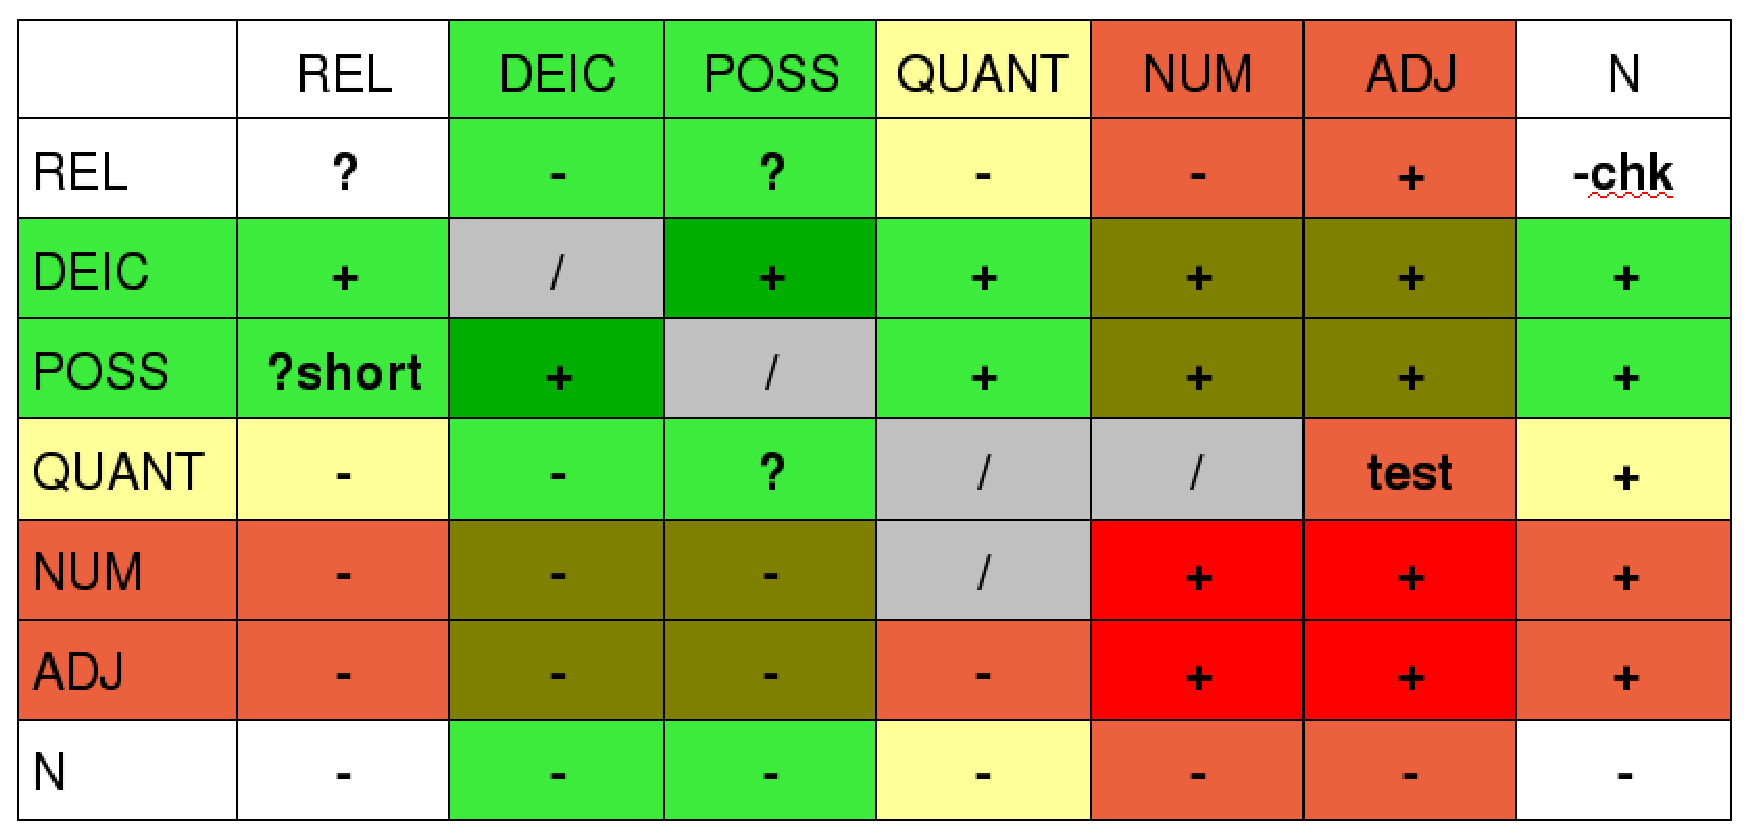
\includegraphics[height=0.3\textwidth]{pics/ModNPtable}
% ModNPtable.eps: 1179666x1179666 pixel, 300dpi, 9987.84x9987.84 cm, bb=14 14 838 400

	\caption[Order of prenominal modifiers]{Order of prenominal modifiers. The cells indicate whether the item at the left end of the row can precede the item at the top of the column. A + indicates that this is possible, a -- indicates that it is impossible, a / indicates that the combination is ruled out semantically, e.g. combination of indefiniteness marker and deictic.}
	\label{tab:OrderOfPrenominalModifiers}
\end{table}
\draftnote{redo table}

The following sections give the logical possibilities and also give an example, if available. Sections without an example indicate that this combination was not found.

\paragraph{RELC RELC N}
It is very difficult to find contexts where a head noun could be modified by two clauses of the Relative Clause type, which comprises both true relative clauses and fact clauses in SLM (see \formref{sec:cls:Relativeclause} for a discussion). Even if this occurs, normally, the two clauses are coordinated and put into \em one \em relative clause, itself consisting of two lower clauses. Example \xref{ex:constr:NP:prenom:relcrelc} shows such a case. The two verbs \trs{mintha}{beg} and \trs{naangis}{cry} both depend on the head noun \trs{swaara}{sound}. But they are found in \em one \em clause.

\xbox{16}{
\ea\label{ex:constr:NP:prenom:relcrelc}
\gll [[Banthu-an asà-mintha]$_{CLS}$  [arà-naangis]$_{CLS}$]$_{RELC}$ [swaara]$_{N}$ hatthu derang=nang su-dìnggar. \\ % bf
      help-\textsc{nmlzr} \textsc{cp}-beg \textsc{simult}-cry sound \textsc{indef} \textsc{3pl}=\textsc{dat} \textsc{past}-hear\\
\z
}\\

To sum up, there is no case of two clauses preceding a head noun as far as syntax is concerned. Semantically speaking, it is possible to have two propositions depending on a head noun, as in \xref{ex:constr:NP:prenom:relcrelc}, but these are packaged into one clause in syntax before they attach to the head noun. The structure is then
[
% 	[
		[
			[...]$_{infinite clause}$ ...
		]$_{finite relative clause}$
% 	]$_{relative clause}$...
]$_{main clause}$


\paragraph{RELC DEIC N}
There is one instance of this order.

\xbox{16}{
\ea\label{ex:constr:NP:prenom:relcdeic}
\gll  [Seelongka   sumniinggal]$_{RELC}$ ithu$_{DEIC}$ thiiga [oorang]$_N$=pe naama kithang thàràthaau. \\ % bf
      Ceylon=\textsc{loc} \textsc{past}-die \textsc{dist} three man=\textsc{poss} name \textsc{1pl} ignore \\
\z
} \\
\paragraph{RELC POSS N}
There is one instance of a possessive pronoun intervening between the relative clause and the head noun, \xref{ex:constr:NP:prenom:relcposs}.

\xbox{16}{
\ea\label{ex:constr:NP:prenom:relcposs}
\gll [ini      {\em British} government=samma pii=apa     mà-oomong]$_{RELC}$ [kithang=pe]$_{POSS}$     [{\em statesmen}]$_{N}$  pada \\ % bf
      \textsc{prox} British government=\textsc{comit} go=after \textsc{inf}-talk \textsc{1pl}=\textsc{poss} statesmen \textsc{pl} \\
\z
} \\
\paragraph{RELC QUANT N}
This order was not found.
\paragraph{RELC NUM N}
The following two examples give this order with a cardinal \xref{ex:constr:NP:prenom:RELCNUM:card} and an ordinal numeral \xref{ex:constr:NP:prenom:RELCNUM:ord}.

\xbox{16}{
\ea\label{ex:constr:NP:prenom:RELCNUM:card}
\gll  [Seelong=ka   sumniinggal]$_{RELC}$ ithu thiiga$_{N}$ [oorang]$_N$=pe naama kithang thàràthaau. \\ % bf
      Ceylon=\textsc{loc} \textsc{past}-die \textsc{dist} three man=\textsc{poss} name \textsc{1pl} ignore \\
\z
} \\
\xbox{16}{
\ea\label{ex:constr:NP:prenom:RELCNUM:ord}
\gll  [{\em terrorist} hatthu=dering  anà-maathi]$_{RELC}$ [kethaama]$_{ADJ}$ oorang$_{N}$=jo    incayang. \\ % bf
      terrorist \textsc{indef}=\textsc{abl} \textsc{past}-die first man=\textsc{foc} \textsc{3s} \\
\z
} \\
\paragraph{RELC ADJ N}
This order is common. There are several instances of it in the corpus. A simple example is \xref{ex:constr:NP:prenom:RELCADJ1}, where \trs{bìssar}{big} is found between the relative clause and the head noun.

\xbox{16}{
\ea\label{ex:constr:NP:prenom:RELCADJ1}
\gll [anà-kijja]$_{RELC}$ [bìssar]$_{ADJ}$  [thumpath]$_{N}$ pada. \\ % bf
 \textsc{past}-make big place pl\\
`The big lands that were made.' (N060113nar02)
\z
}

\em Bìssar \em is also found as the intervening adjective in \xref{ex:constr:NP:prenom:RELCADJ2}.

\xbox{16}{
\ea\label{ex:constr:NP:prenom:RELCADJ2}
\gll [sithu=ka     aada]$_{RELC}$  [bìssar]$_{ADJ}$ [oorang]$_{N}$ pada=yang   asà-{\em attack}-kang     {\em mail}=nya    asà-cuuri {\em mail}=ka    duwith arà-baapi. \\ % bf
     there=\textsc{loc} exist big man \textsc{pl}=\textsc{acc} \textsc{cp}-attack-\textsc{caus} mail=\textsc{acc} \textsc{cp}-steal mail=\textsc{loc} money \textsc{simult}-bring  \\
\z
} \\
The head of a relative clause does not have to be a noun actually, an interrogative pronoun is possible as well, as shown in \xref{ex:constr:NP:prenom:RELCADJ4}, where additionally the adjective \trs{lai}{other} intervenes between the relative clause and the interrogative pronoun.

\xbox{16}{
\ea\label{ex:constr:NP:prenom:RELCADJ4}
\gll incalla   [lai     thaau sudaara sudaari pada]=ka    bole=caanya    ambel [nya-gijja]$_{RELC}$    [lai]$_{ADJ}$     [saapa=kee]$_{HEAD}$  aada=si    katha]. \\ % bf
      Hopefully other know brother sister \textsc{pl}=\textsc{loc} can-ask take \textsc{past}-make other who=\textsc{simil} exist=\textsc{interr} \textsc{quot} \\
\z
} \\
A somewhat different case is given in \xref{ex:constr:NP:prenom:RELCADJ:purp}, where we are dealing with a purposive clause, which precedes the adjective.

\xbox{16}{
\ea\label{ex:constr:NP:prenom:RELCADJ:purp}
\gll  kithang lorang=nang baaye mliiga athi-kaasi, [mà-kaaving]$_{RELC}$ [panthas]$_{ADJ}$ [pompang]$_{N}$ pada athi-kaasi,  duwith athi-kaasi. \\ % bf
      \textsc{1pl} \textsc{2pl}=\textsc{dat} good palace \textsc{irr}-give \textsc{inf}-marry beautiful female \textsc{pl} \textsc{irr}-give money \textsc{irr}-give \\
\z
} \\

% \xbox{16}{
% \ea\label{ex:constr:NP:prenom:RELCADJ}
% \gll  laayeng [kithang=nang   aada]$_{RELC}$  [laayeng]$_{ADJ}$  [makanan]$_{N}$        pada saathe. \\
%       other \textsc{1pl}=\textsc{dat} exist other food \textsc{pl} sate \\
%     `Another dish we have is sate.' (K061026rcp03)
% \z
% } \\

% \xbox{16}{
% \ea\label{ex:constr:NP:prenom:RELCADJ}
% \gll  ini [kuurang arà-duuduk]$_{RELC}$     [laayeng]$_{ADJ}$  [kumpulan]$_{N}$   pada=yang   mà-{\em represent}-kang=nang. \\
%       \textsc{prox} few \textsc{non.past}-exist.\textsc{anim} other group \textsc{pl}=\textsc{acc} \textsc{inf}-represent-\textsc{caus}=\textsc{dat} \\
% \z
% } \\


\paragraph{RELC N N}
This order was not found.

\paragraph{DEIC RELC      N}
Both the proximal \xref{ex:constr:NP:prenom:deicrelc:ini} and the distal deictic \xref{ex:constr:NP:prenom:deicrelc:ithu} have been found to precede a relative clause.

 \xbox{16}{
\ea\label{ex:constr:NP:prenom:deicrelc:ini}
   \gll  incayang  [ini]$_{DEIC}$    [Seelong=ka  anà-aada]$_{RELC}$    [lakuan]$_{N}$   [baathu]$_{N}$ asà-caari. \\ % bf
    \textsc{3s.polite} \textsc{prox} Seelon=\textsc{loc} \textsc{past}-exist wealth stone \textsc{cp}-find \\
\z
}

 \xbox{16}{
\ea\label{ex:constr:NP:prenom:deicrelc:ithu}
   \gll  [ithu]$_{DEIC}$     [spaaman anà-niinggal]$_{RELC}$   [thumpath]$_{N}$=nang=le        [Passara   katha  arà-biilang    nigiri]=nang=le   dìkkath. \\ % bf
    \textsc{dist} \textsc{3s.polite} \textsc{past}-die place=\textsc{dat}=\textsc{addit} Passara \textsc{quot} \textsc{non.past}-say village=\textsc{dat}=\textsc{addit} vicinity\\
\z
}

\paragraph{DEIC DEIC N}
This order was not found.

\paragraph{DEIC POSS N}
The deictics can be found preceding a possessor and a noun.

\xbox{16}{
\ea\label{ex:constr:NP:prenom:DEICPOSSN1}
\gll [ini]$_{DEIC}$ [indonesia=pe]$_{POSS}$ [oorang]$_{N}$=si giithu kaltraa {\em Malaysian} oorang=si. \\ % bf
     \textsc{prox} Indonesia=\textsc{poss} man=disj that.way ifnot Malaysian man=disj  \\
    `These Indonesians or otherwise Malaysians.'  (K060108nar02)
\z
}\\


\xbox{16}{
\ea\label{ex:constr:NP:prenom:DEICPOSSN2}
\gll  11th=ka su-aada [itthu]$_{DEIC}$ [kithang=pe igaama=pe]$_{POSS}$       [mosthor]$_{N}$=nang. \\ % bf
     11th=\textsc{loc} \textsc{past}-exist \textsc{dist} \textsc{1pl}=\textsc{poss} religion=\textsc{poss} manner=\textsc{dat}  \\
\z
} \\
\paragraph{DEIC QUANT N}
Deictics and quantifiers precede the noun, in that order.

\xbox{16}{
\ea\label{ex:constr:NP:prenom:DEICQUANTN}
\gll {\em school}=nang arà-pii=subbath=jo [inni]$_{DEIC}$ [samma]$_{QUANT}$ [seksa]$_{N}$. \\ % bf
    school=\textsc{dat} \textsc{non.past}-go=because=\textsc{foc} \textsc{prox} all problems   \\
\z
}\\

\paragraph{DEIC NUM N}
Deictics and numeral precede the noun, in that order.

\xbox{16}{
\ea\label{ex:constr:NP:prenom:DEICNUMN}
\gll  [ini]$_{DEIC}$ [duuwa]$_{NUM}$ [{\em army}]$_{N}$ [{\em captain}]$_{N}$ thàrà-maathi. \\ % bf
       \textsc{prox} two army captain \textsc{neg.past}-dead\\
    `These two army captains did not die.' (K051213nar06)
\z
} \\
\paragraph{DEIC ADJ N}
Deictics precede the adjective in the noun phrase.

\xbox{16}{
\ea\label{ex:constr:NP:prenom:DEICADJN}
\gll [ini]$_{DEIC}$ [laama]$_{adj}$ [\em {\em car}]$_{N}$ pada=jo kithang arà-baapi. \\ % bf
      \textsc{prox} old car \textsc{pl}=\textsc{foc} \textsc{1pl} \textsc{non.past}-bring \\
\z
}\\

% \xbox{16}{
% \ea\label{ex:constr:NP:unreferenced}
% \gll derang anà-cuuri  bae      [nni]$_{DEIC}$       [kaaya]$_{ADJ}$ oorang$_{N}$ pada=dering. \\
%     \textsc{3pl} \textsc{past}-steal    good     \textsc{prox} rich man \textsc{pl}=\textsc{abl}  \\
% \z
% }\\


% \xbox{16}{
% \ea\label{ex:constr:NP:unreferenced}
% \gll itthu    baapa=le      ithukang       ithu    kiccil aanak=le     asà-baa. \\
%      \textsc{dist} father=\textsc{addit} then \textsc{dist} small child=\textsc{addit} \textsc{cp}-bring  \\
% \z
% } \\

\paragraph{DEIC N N}
The following two examples show deictics preceding two nouns. If these strings of two nouns are analyzed as syntactic combinations, we get the sequence DEIC N N, i.e. a deictic preceding a noun modifying a noun.


\xbox{16}{
\ea\label{ex:constr:NP:prenom:DEICN:righthead:1}
\gll kitham=pe=le   [inni]$_{DEIC}$   [prompang]$_{N}$ [kumpulan]$_{N}$    bannyak samma=ka    arà-banthu. \\ % bf
      \textsc{1pl}=\textsc{poss}=\textsc{addit} \textsc{prox} woman association much every=\textsc{loc} \textsc{non.past}-help \\
\z
}\\


\xbox{16}{
\ea\label{ex:constr:NP:prenom:DEICN:righthead:2}
\gll aapcara=ke       incayang  [ini]$_{DEIC}$ [ciina]$_{N}$ [oorang]$_{N}$ islam=nang   asà-dhaathang  asà-kaaving=apa=  karang mà-siigith=nang  arà-pii. \\ % bf
     how=\textsc{simil} \textsc{3s.polite} \textsc{prox} China man Islam=\textsc{dat} \textsc{cp}-come \textsc{cp}-marry=after now mosque=\textsc{dat} \textsc{non.past}-go  \\
\z
} \\
\paragraph{POSS RELC    N}
Very short relative clauses can be preceded by a possessor, as in \xref{ex:constr:NP:prenom:POSSRELC}, where the possessor \trs{se=ppe}{my} immediately precedes the relative clause \trs{nya-laaher}{being born}. Note that this example has a lot of code-mixing with English in it, so that its value could be contested.

\xbox{16}{
\ea\label{ex:constr:NP:prenom:POSSRELC}
\gll  [se=ppe]$_{POSS}$ [nya-laaher]$_{RELC}$ [{\em date}]$_{N}$ duuwa duuwa 1960. \\ % bf
     \textsc{1s}=\textsc{poss} \textsc{past}-be.born date two two 1960  \\
\z
} \\
% \xbox{16}{
% \ea\label{ex:constr:NP:unreferenced}
% \gll [itthu=pe]$_{POSS}$        [nya-puunya]$_{RELC}$ \zero$_{HEAD}$. \\
%      \textsc{dist}=\textsc{poss} \textsc{past}-own  \\
% \z
% } \\

\paragraph{POSS DEIC N}
Normally, the location of possessed items is retrievable for the hearer, and the deictics \em ini \em and \em itthu \em do not combine with possessed items then. In the following two examples, the deictics are used for emphasis.

\xbox{16}{
\ea\label{ex:constr:NP:prenom:POSSDEICN1}
\gll Kandi=pe     raaja=nang   [kitham=pe]$_{POSS}$ [inni]$_{DEIC}$     [banthu-an]$_{N}$  asà-kamauwan      se-aada. \\ % bf
     Kandy=\textsc{poss} king=\textsc{dat} \textsc{1pl}=\textsc{poss} \textsc{prox} help-nmlz \textsc{cp}-want \textsc{past}-exist  \\
\z
} \\
\xbox{16}{
\ea\label{ex:constr:NP:prenom:POSSDEICN2}
   \gll    [kithang=pe]$_{POSS}$  [ini]$_{DEIC}$      pompang$_{N}$ kumpulan$_{N}$      bannyak samma=nang   arà-banthu. \\ % bf
    \textsc{1pl}=\textsc{poss} \textsc{prox} female association much all=\textsc{dat} \textsc{non.past}-help \\
\z
}

In examples \xref{ex:constr:NP:prenom:POSSDEICN3}, the possessor is used to recall that the Malays being talked about are actually forefathers of the speaker.

\xbox{16}{
\ea\label{ex:constr:NP:prenom:POSSDEICN3}
\gll  Indonesia=dering Sri Lanka=nang [kithang=pe]$_{POSS}$ [ini]$_{DEIC}$ [mlaayu]$_{N}$ pada asà-dhaathang ini {\em Malay} {\em regiment} atthu. \\ % bf
      Indonesia=\textsc{abl} Sri Lanka=\textsc{dat} \textsc{1pl}=\textsc{poss} \textsc{prox} Malay \textsc{pl} \textsc{cp}-come \textsc{prox} Malay regiment \textsc{indef} \\
\z
} \\
\paragraph{POSS POSS N}
There is strictly speaking no modification of a noun by two possessors, since an item normally has only one possessor. What is possible is recursive possession, but this is not a modification of one head noun by several possessors, but a modification of the head noun on level N-1 by the possessor on level N \xref{ex:constr:NP:pepe1}\xref{ex:constr:NP:pepe2}.

\xbox{16}{
\ea\label{ex:constr:NP:pepe1}
\gll  [se=ppe$_{POSS}$      dhaatha]$_{N}$=pe]$_{POSS}$          thiiga [aanak]$_{N}$=le      Dubai=ka     arà-duuduk. \\ % bf
 \textsc{1s}=\textsc{poss} elder.sister=\textsc{poss} three child=\textsc{addit} Dubai=\textsc{loc} \textsc{non.past}=stay\\
\z
}

\xbox{16}{
\ea\label{ex:constr:NP:pepe2}
\gll  [[se=ppe$_{POSS}$ bìssar aade]$_{N}$]=pe]$_{POSS}$  manthu. \\ % bf
      \textsc{1s}=\textsc{poss} big younger.sibling=\textsc{poss} child.in.law \\
    `My elder younger brother's son-in-law.'  (K060116nar02.21 )
\z
}\\



\paragraph{POSS QUANT N}

This order of prenominal modifiers is possible and is given in the following three examples.

\xbox{16}{
\ea\label{ex:constr:NP:prenom:POSSQUANTN1}
\gll itthu blaakang [kithang=pe]$_{POSS}$     [bannyak]$_{QUANT}$ sudaari$_{N}$ sudaara$_{N}$ pada,  kithang anà-pii    ruma  saakith=nang. \\ % bf
     \textsc{dist} after \textsc{1pl}=\textsc{poss} much sister brother \textsc{1pl} \textsc{past}-go house sick=\textsc{dat}  \\
\z
} \\
\xbox{16}{
\ea\label{ex:constr:NP:prenom:POSSQUANTN2}
\gll  [ini kaaving=nang aada] haadath-saadath pada, [kitham=pe]$_{POSS}$ bannya$_{QUANT}$ [ooram]$_{N}$ pada arà-kijja. \\ % bf
     \textsc{prox} wedding=\textsc{dat} exist   traditions \textsc{pl} 1p=\textsc{poss} many people \textsc{pl} \textsc{non.past}-make\\
\z
}\\



\xbox{16}{
\ea\label{ex:constr:NP:prenom:POSSQUANTN3}
   \gll  derang=nang   [Kluumbu=pe]$_{POSS}$    [samma]$_{QUANT}$ [{\em association}]$_{N}$=le      {\em support}. \\ % bf
    \textsc{3pl}=\textsc{dat} Colombo=\textsc{poss} all association=\textsc{addit} support \\
`All Colombo associations supported them.' (K060116nar06)5.11.08
\z
}

\paragraph{POSS NUM N}
This order is given in the following two examples.

\xbox{16}{
\ea\label{ex:constr:NP:prenom:POSSNUMN1}
\gll  [mliige=pe]$_{POSS}$     [duuwa]$_{NUM}$ [subla]$_{N}$=ka su-thaanam. \\ % bf
       palace=\textsc{poss} two side=\textsc{loc} \textsc{past}-plant \\
\z
} \\
\xbox{16}{
\ea\label{ex:constr:NP:prenom:POSSNUMN2}
\gll  se=ppe   [dhaatha=pe]$_{POSS}$  [thiiga]$_{NUM}$ [aanak]$_{N}$=le  Dubai=ka     arà-duuduk. \\ % bf
 \textsc{1s}=\textsc{poss} elder.sister=\textsc{poss} three child=\textsc{addit} Dubai=\textsc{loc} \textsc{non.past}=stay\\
\z
}

\paragraph{POSS ADJ N}
The possessor can precede the adjective preceding a noun.

\xbox{16}{
\ea\label{ex:constr:NP:prenom:POSSADJN1}
\gll  [se=ppe]$_{POSS}$ [bìssar]$_{ADJ}$ [aade]$_{N}$=pe  manthu. \\ % bf
      \textsc{1s}=\textsc{poss} big younger.sibling=\textsc{poss} child.in.law \\
    `My elder younger brother's son-in-law.'  (K060116nar02.21 )
\z
}\\

\xbox{16}{
\ea\label{ex:constr:NP:prenom:POSSADJN2}
\gll itthu=le [oorang mlaayu=pe]$_{POSS}$ [baaye]$_{ADJ}$ hathu [{\em traditional} {\em food}]$_{N}$ hatthu. \\ % bf
      \textsc{dist}=\textsc{addit} man Malay=\textsc{poss} good \textsc{indef} tradtional food \textsc{indef} \\
\z
} \\
\paragraph{POSS N N}
A possessor can precede a sequence of two nouns.

\xbox{16}{
\ea\label{ex:constr:NP:prenom:POSSNN}
\gll [se=ppe]$_{POSS}$ [aanak]$_{N}$ [pompang]$_{N}$=nang duuwa aanak klaaki. \\ % bf
     \textsc{1s}=\textsc{poss} child female=\textsc{dat} two child male  \\
    `My daughter has two sons.'  (K051201nar01)
\z
}\\

\paragraph{QUANT RELC N}
This order was not found.

\paragraph{QUANT DEIC N}
This order was not found.

\paragraph{QUANT POSS N}
The noun can be preceded by a quantifier and a possessor in that order.

\xbox{16}{
\ea\label{ex:constr:NP:prenom:quantposs}
\ea
   \gll  samma oorang {\em school}=nang   asà-pii   arà-blaajar    cinggala. \\  % bf
    all   man   school=\textsc{dat} \textsc{cp}-go \textsc{non.past}-learn Sinhala \\
\ex
   \gll  [samma]$_{QUANT}$ [kithang=pe]$_{POSS}$     [mlaayu]$_{N}$, hathu  muusing su-aada,      samma cinggala=dering=jo      athi-oomong. \\
    all   \textsc{1pl}=\textsc{poss} Malay  \textsc{indef}  time    \textsc{past}-exist all   Sinhalese=\textsc{abl}=\textsc{foc} \textsc{irr}-talk \\
\z
\z
}

\paragraph{QUANT QUANT N}
This order was not found.

\paragraph{QUANT NUM N}
This order was not found.

\paragraph{QUANT ADJ N}

The quantifier precedes the adjective, as shown in the following example.


\xbox{16}{
\ea\label{ex:constr:NP:prenom:QUANTADJN}
\gll spaaru bìssar ruuma pada aada. \\
      some big house \textsc{pl} exist \\
    `There are some big houses.'  (test)5.11.08 OK
\z
}\\




\paragraph{QUANT N N}
A quantifier can precede a string of two nouns, as shown in the following example.


\xbox{16}{
\ea\label{ex:constr:NP:prenom:quantn}
\gll Derang derang=pe  umma=nang butthul saayang=kee=jo [samma]$_{QUANT}$ [ruuma]$_{N}$ [pukurjan]$_{N}$=nang=le anà-banthu. \\ % bf
 \textsc{3pl} \textsc{3pl}=\textsc{poss} mother=\textsc{dat} correct love=\textsc{simil}=\textsc{foc} all house work=\textsc{dat}=\textsc{addit} \textsc{past}-help  \\
\z
}\\


%
% \xbox{16}{
% \ea\label{ex:constr:NP:prenom:quantn}
% \gll bannyak$_{QUANT}$ Muslim$_{N}$ oorang$_{N}$ pada araduuduk. \\
%      many Muslim man \textsc{pl} \textsc{non.past}-exist.\textsc{anim}  \\
% \z
% } \\
\paragraph{NUM   RELC  N}
This order was not found.
\paragraph{NUM   DEIC N}
This order was not found.
\paragraph{NUM   POSS N}
This order was not found.
\paragraph{NUM   QUANT N}
This order was not found.
\paragraph{NUM   NUM N}

A head noun can be modified by two adjacent numerals, which conveys uncertainty about the exact amount.
In the following example, the speaker is not sure whether his stay in the Navy lasted twelve or thirteen years. The two numeral \trs{doblas}{twelve} and \trs{thigablas}{thirteen} jointly modify the noun.

\xbox{16}{
\ea\label{ex:constr:NP:prenom:NUMNUMN}
\gll Oman      {\em Navy}=ka    se-duuduk hatthu [doblas]$_{NUM}$  [thiga-blas]$_{NUM}$ [thaaun]$_{year}$=ke. \\ % bf
     Oman Navy=\textsc{loc}      \textsc{past}-stay   one   twelve   three-teen year=simil\\
    `I stayed in the Oman Navy for about 12 or thirteen years, something like that.'  (K051206nar17)
\z
}\\

However, it could be argued that in this case, we are not dealing with two modifications, but rather with one complex modification. It is not the case that the years had a cardinality of twelve and that the years at the same time had a cardinality of thirteen. Rather, they had only one cardinality, which is vague and therefore expressed by the complex numeral modifier [doblas thigablas]$_{NUM}$.

\paragraph{NUM ADJ N}

\xbox{16}{
\ea\label{ex:constr:NP:prenom:NUMADJN}
\gll thiiga kiccil aanak pada aada. \\
       \\
    `.'  (test)OK 5.11.08
\z
}\\

\paragraph{NUM N N}
A string of two nouns can be preceded by a numeral.

\xbox{16}{
\ea\label{ex:constr:NP:prenom:NUMNN}
\gll se=dang duuwa$_{NUM}$ pompang$_{N}$ aade$_{N}$=le hathu$_{NUM}$ klaaki$_{N}$ aade$_{N}$=le anà-duuduk. \\ % bf
     \textsc{1s=dat} two woman younger.sibling=\textsc{addit} one man younger.sibling=\textsc{addit} \textsc{past}-exist  \\
\z
}\\
%
%  \xbox{16}{
%  \ea\label{ex:constr:NP:unreferenced}
%    \gll se=dang duuwa   aade  [duuwa]$_{NUM}$ klaaki$_{N}$   aade$_{N}$ pada=le hatthu  pompang aade=le   arà-duuduk. \\
% \textsc{1s=dat} two younger.sibling two male younger.sibling \textsc{pl}=\textsc{addit} one female  younger.sibling=\textsc{addit} \textsc{non.past}-exist.\textsc{anim}\\
% \z

%army captain

\paragraph{ADJ   RELC  N}
This order was not found.
\paragraph{ADJ   DEIC N}
This order was not found.
\paragraph{ADJ   POSS N}
This order was not found.
\paragraph{ADJ   QUANT N}
This order was not found.

\paragraph{ADJ   NUM N}
Very rarely, a numeral can be found between an adjective and its head noun.

\xbox{16}{
\ea\label{ex:constr:NP:prenom:ADJNUMN1}
\gll [mlaayu]$_{ADJ}$ [thiga-pulu tuuju]$_{NUM}$ [baasa]$_{N}$    aada. \\ % bf
 Malay three-ty seven language exist\\
`There are 37 Malay languages [in the world].' (K060116nar02)
\z
}

While above, we are dealing with a genuine adjective, the two examples below show this pattern with \trs{hathyang}{next} and \trs{lai}{additional}, where it can be argued that the scope relations are slightly different, similar to English \em Another three men\em, as compared to \em three other men\em.

\xbox{16}{
\ea\label{ex:constr:NP:prenom:ADJNUMN2}
\gll [hathyang]$_{ADJ}$ [thiiga]$_{NUM}$ [oorang]$_{N}$=yang {\em Malaysia}=nang su-ambel baapi. \\ % bf
     next three man=\textsc{acc} Malaysia=\textsc{dat} \textsc{past}-take bring \\
\z
}\\

\xbox{16}{
\ea\label{ex:constr:NP:prenom:ADJNUMN3}
\gll  kitham=nang duppang [lai]$_{ADJ}$ [duuwa]$_{NUM}$ [bàrgaada]$_{N}$ asà-dhaathang aada. \\ % bf
 \textsc{1pl}=\textsc{dat} before additional two group \textsc{non.past}-come exist \\
`Before us, there are two more families.' (K060108nar02)
\z
}

\paragraph{ADJ ADJ N}
Two adjectives can stack before a noun. \draftnote{bad example}


\xbox{16}{
\ea\label{ex:constr:NP:prenom:ADJADJN}
\gll   se=ppe bìssar$_{ADJ}$ lai$_{ADJ}$ ruuma$_{N}$ aada. \\ % bf
       \textsc{1s}=\textsc{poss}     big    other  house exist\\
    `There is another big house of mine.'  (B060115cvs09.7)
\z
}\\

%K060116nar06.50  inni     katha sin        bae  kiccil atthu    pukkjang


\paragraph{ADJ   N N}
An adjective can precede a string of two \xref{ex:constr:NP:prenom:adjn:two} or more  nouns \xref{ex:constr:NP:prenom:adjn:two}.


\xbox{16}{
 \ea\label{ex:constr:NP:prenom:adjn:two}
   \gll  suda se=ppe    [thuuwa]$_{ADJ}$ [anak]$_{N}$  [klaaki]$_{N}$ asadhaathang dhlapan-blas    thaaun. \\  % bf
     so \textsc{1s}=\textsc{poss} old child male \textsc{copula} eight-teen year \\
`So my eldest son is eighteen' (K060108nar02)
\z
}

\xbox{16}{
 \ea\label{ex:constr:NP:prenom:adjn:more}
\gll [panthas]$_{ADJ}$ [rooja]$_{N}$  [kumbang]$_{N}$   [pohong]$_{N}$  [komplok]$_{N}$ duuwa  asà-jaadi su-aada. \\ % bf
      beautiful rose flower tree bush two \textsc{cp}-grow \textsc{past}-exist \\
    `Two beautiful rose bushes had grown.'  (K070000wrt04)
\z
}\\




\paragraph{N RELC  N}
This order was not found.
\paragraph{N DEIC N}
This order was not found.
\paragraph{N POSS N}
This order was not found.
\paragraph{N QUANT N}
This order was not found.
\paragraph{N NUM N}
This order was not found.
\paragraph{N ADJ N}
This order was not found.


\paragraph{N N N}
Strings of three or more nouns are also possible

\xbox{16}{
\ea\label{ex:constr:NP:prenom:NNN}
\gll  panthas  [rooja]$_{N}$  [kumbang]$_{N}$ [pohong]$_{N}$  [komplok]$_{N}$ duuwa asà-jaadi su-aada. \\ % bf
      beautiful rose flower tree bush two \textsc{cp}-grow \textsc{past}-exist \\
    `Two beautiful rose bushes had grown.'  (K070000wrt04)
\z
}\\

\subsection{Preliminary summary of prenominal modifications}\label{sec:nppp:Preliminarysummaryofprenominalmodifications}

We can schematize the findings about prenominal modifications as in \xref{cb:np:prenom}

\cb[\label{cb:np:prenom}]{
RELC
$\left\{\begin{array}{l} \rm DEIC\\\rm POSS\end{array}\right\}$
QUANT
$\left\{\begin{array}{l} \rm NUM\\\rm ADJ\end{array}\right\}$*
Noun
}

Up to now, we have omitted discussion of the position of the indefiniteness marker \em (h)a(t)thu\em. The position of this marker within the NP will be discussed in the next section.

\subsection{The position of the indefinite modifier}\label{sec:nppp:Thepositionoftheindefinitemodifier}
Above, we have treated the order of some prenominal modifiers. There is one modifier which we have not treated, which is the indefiniteness marker \em atthu\em. This marker can intervene between any two markers in \xref{cb:np:prenom}, and additionally can also occur more than once. Example \xref{ex:constr:NP:atthu:triple} gives a sentence with multiple occurrence of \em atthu \em in one NP. The possibility to occur more than once points to an appositional nature of the NP, which will be discussed in more detail in \formref{sec:nppp:TheSLMNPasappositional}.

\xbox{16}{
\ea\label{ex:constr:NP:atthu:triple}
\gll itthu=le \textbf{hathu}  mlaayu oorang pada=pe \textbf{hathu}  baae \textbf{hathu} makanan=jo. \\ % bf
     \textsc{dist}=\textsc{addit} \textsc{indef} Malay man \textsc{pl}=\textsc{poss} \textsc{indef} good \textsc{indef} food=\textsc{foc}  \\
\z
} \\


\paragraph{\em hatthu \em preceding a relative clause}
This order was not found.


\paragraph{\em hatthu \em following a relative clause}

The following three examples show the use of \em atthu \em after a subordinate clause modifying the noun. This is a relative clause in \xref{ex:constr:NP:prenom:atthu:relc:follow1} and \xref{ex:constr:NP:prenom:atthu:relc:follow2} and a purposive clause in \xref{ex:constr:NP:prenom:atthu:relc:follow3}.

\xbox{16}{
\ea\label{ex:constr:NP:prenom:atthu:relc:follow1}
\gll [anà-birthi-king]$_{RELC}$ hatthu$_{INDEF}$ paapang$_{N}$=ka. \\ % bf
      \textsc{past}-stand-\textsc{caus} \textsc{indef} pole=\textsc{loc} \\
\z
}\\  5.11.08

\xbox{16}{
\ea\label{ex:constr:NP:prenom:atthu:relc:follow2}
\gll [kìrras pinthu=nang arà-thatti]$_{RELC}$ hathu$_{INDEF}$=swaara$_{N}$ su-dìnggar. \\ % bf
     strong door=\textsc{dat} \textsc{simult}-hammer] \textsc{indef}=noise \textsc{past}-hear \\
\z
}\\


\xbox{16}{
\ea\label{ex:constr:NP:prenom:atthu:relc:follow3}
\gll pohong jaatho=nang   blaakang jleena=pe     dìkkath=nang    asà-dhaathang [thaangang  mà-saapu]$_{RELC}$    hatthu$_{INDEF}$ {\em paper}$_{N}$ kapang-mintha  baapa-yang       su-kuthumung,     dee {\em bed}=ka. \\ % bf
    tree fall=\textsc{dat} after window=\textsc{poss} vicinity=\textsc{dat} \textsc{cp}-come hand \textsc{inf}-sweep one paper when-ask father-hyperch \textsc{past}-see \textsc{3s} bed=\textsc{loc}   \\
\z
} \\
%  \xbox{16}{
% \ea\label{ex:constr:NP:prenom:atthu:relc:follow4}
%    \gll  go  [bannyak pasiyeth   nya-baapi]$_{RELC}$   [hathu]$_{INDEF}$  oorang$_{N}$ \\ %     \textsc{1s}  {\em much}   {\em trouble} \textsc{past}-{\em bring} \textsc{indef} man. \\
% \z
% }
%
% \xbox{16}{
% \ea\label{ex:constr:NP:prenom:atthu:relc:follow5}
% \ea
% \gll inni     pukujan=nang  kam-pii. \\
%      \textsc{prox} work=\textsc{dat} when-go \\
%    `When they go to this work.'
% \ex
% \gll  deram pada [itthu makumpul]]$_{RELC}$ [hatthu=]$_{INDEF}$ [mosthor]$_{N}$ thraa. \\
% \textsc{3pl} \textsc{dist} \textsc{inf}-add \textsc{indef}=manner neg\\
% \z
% \z
% } \\
\paragraph{\em hatthu \em following or preceding a deictic}
given the semantics of \em hatthu \em marking indefiniteness, and the deictics marking definite referents, these morphemes cannot cooccur.

\paragraph{\em hatthu \em preceding a possessor}

\em hatthu \em can precede the possessor \xref{ex:constr:NP:prenom:atthu:poss:prec}, but is more likely to follow it as will be discussed in the next section

\xbox{16}{
\ea\label{ex:constr:NP:prenom:atthu:poss:prec}
\gll itthu=le [hathu]$_{INDEF}$  [mlaayu oorang pada=pe]$_{POSS}$ hathu baae hathu [makanan]$_{N}$=jo. \\ % bf
     \textsc{dist}=\textsc{addit} \textsc{indef} Malay man \textsc{pl}=\textsc{poss} \textsc{indef} good \textsc{indef} food=\textsc{foc}  \\
\z
} \\
\paragraph{\em hatthu \em following a possessor}

To indicate that within a set of possessed items, an indefinite one is talked about, \em atthu \em and the possessor can cooccur. In those cases, \em atthu \em normally follows the possessor. In example \xref{ex:constr:NP:atthu:poss:follow1}, the speaker has many sons, but only one of them, who is at the time of speaking not known to the hearer, is on the estates.

\xbox{16}{
\ea\label{ex:constr:NP:atthu:poss:follow1}
\gll karang [se=ppe]$_{POSS}$    hathu$_{INDEF}$  aanak$_{N}$ {\em estate}=ka. \\ % bf
     now \textsc{1s=poss} \textsc{indef} child estate=\textsc{loc}  \\
\z
}

Similar things can be said about \xref{ex:constr:NP:atthu:poss:follow2}, where the identity of the Malay woman's child is unknown to the hearer.

\xbox{16}{
\ea\label{ex:constr:NP:atthu:poss:follow2}
\gll lai=le  hatthu  [sudaari=pe]$_{POSS}$ atthu$_{INDEF}$ aanak$_{N}$, kiccil aanak atthu  puruth=ka    se-mniinggal. \\ % bf
 more=\textsc{addit} \textsc{indef} sister=\textsc{poss} \textsc{indef} child small child \textsc{indef} womb=\textsc{loc} \textsc{past}-die  \\
\z
}\\

The third example for this patterns has again to do with indicating that the speaker is not supposed to be able to identify which one of the children the speaker is talking about.


\xbox{16}{
\ea\label{ex:constr:NP:atthu:poss:follow3}
\gll   [itthu    kaake=pe]$_{POSS}$          [hatthu]$_{INDEF}$ [aanak]$_{N}$=jo    se=ppe    umma. \\ % bf
      \textsc{dist} grandfather=\textsc{poss} once child=\textsc{foc} \textsc{1s=poss} mother \\
\z
}
%
% \xbox{16}{
% \ea\label{ex:constr:NP:atthu:poss:follow1}
% \gll maana=ke hathu [government=pe]$_{POSS}$   [hathu]$_{INDEF}$   [thumpath]$_{N}$ =ka    asà-pii   pukurjan bole=girja. \\
%     where=\textsc{simil} \textsc{indef} government=\textsc{poss} \textsc{indef} place=\textsc{loc} \textsc{cp}-go work can-do   \\
% \z
% } \\


\paragraph{\em hatthu \em following or preceding a quantifier}
These orders were not found.
\paragraph{\em hatthu \em preceding a numeral}
\em hatthu \em can precede a numeral, in which case it marks uncertainty about the exact amount. Still, this is an instance of \em hatthu \em modifying the numeral expression rather than the noun.

\xbox{16}{
\ea\label{ex:constr:NP:prenom:INDEFNUMN}
\gll Oman {\em Navy}=ka se-duuduk  [hatthu$_{INDEF}$ doblas$_{NUM}$  thiga-blas$_{NUM}$]$_{NUM}$ [thaaun]$_{N}$=ke. \\ % bf
     Oman         Navy=\textsc{loc}       \textsc{past}-stay   \textsc{indef}   twelve   three-teen year=simil\\
    `I stayed in the Oman Navy for about 12 or thirteen years, something like that.'  (K051206nar17)
\z
}\\

\paragraph{\em hatthu \em following a numeral}
This order was not found.

\paragraph{\em hatthu \em preceding an adjective}
\em hatthu \em can precede an adjective modifying a noun.


\xbox{16}{
\ea\label{ex:constr:NP:prenom:INDEFADJN}
\gll Hathu muusing=ka ...  [hathu]$_{INDEF}$  [kiccil]$_{ADJ}$ [ruuma]$_{N}$ su-aada \\
     \textsc{indef} time=\textsc{loc} ... \textsc{indef} small house \textsc{past}-exist  \\
    `Once upon a time, there was a small house.'  (K07000wrt04)
\z
}\\


% \xbox{16}{
% \ea\label{ex:constr:NP:prenom:INDEFADJN}
% \gll  samma hatthu$_{INDEF}$ bae$_{ADJ}$  kumpulan$_{N}$    an-duuduk. \\ % bf
%       every \textsc{indef} good association \textsc{past}-stay \\
%     `They all stayed together as one association'  (K060116nar02.16)
% \z
% }\\
%
% \xbox{16}{
% \ea\label{ex:constr:NP:prenom:}
% \gll {\em majority} katha arà-biilang hathu$_{INDEF}$ liiwath$_{ADJ}$ blaangan$_{N}$ {\em votes}=dering su-bunnang. \\ % bf
%      majority \textsc{quot} \textsc{non.past}-say \textsc{indef} excessive amount votes=\textsc{abl} \textsc{past}-win \\
% \z
% }\\



\paragraph{\em hatthu \em following an adjective}
Just like \em atthu \em can precede the adjective, it can also follow, as shown in \xref{ex:constr:NP:prenom:ADJINDEFN}.

% \xbox{16}{
% \ea
% \gll blaakang se=dang=jo        [kiccil] [hatthu] [seksa]  hatthu se-jaadi. \\ % bf
%      after \textsc{1s=dat} small \textsc{indef} problem \textsc{indef} \textsc{past}-become  \\
% \z
% }\\

\xbox{14}{
\ea \label{ex:constr:NP:prenom:ADJINDEFN}
\gll  Itthu [bannyak [laama]$_{ADJ}$ [hathu]$_{INDEF}$ [ruuma]$_{N}$]. \\ % bf
      \textsc{dist} very old \textsc{indef} house \\
    `That one was a very old house.'  (K070000wrt04)
\z
}\\

\paragraph{\em hatthu \em preceding a modifying noun}

It is the normal case for \em atthu \em to precede a modifying noun.

\xbox{16}{
\ea\label{ex:constr:NP:prenom:INDEFNN}
\gll sithu=ka, [hathu]$_{INDEF}$ bìssar [beecek caaya]$_{N}$ [Buruan]$_{N}$  su-duuduk.\\ % bf
     there=\textsc{loc} \textsc{indef} big mud colour bear \textsc{past}-exist \\
\z
}\\


\paragraph{\em hatthu \em following a modifying noun}

In some instances, \em atthu \em can intervene between the two nouns of a two-noun sequence. The following two examples show this for a monkey group and a street bend.

\xbox{16}{
\ea\label{ex:constr:NP:prenom:NINDEFN1}
\gll Ini pohong atthas=ka [moonyeth]$_{N}$ [hathu]$_{INDEF}$=[kawanan]$_{N}$ su-aada. \\ % bf
     \textsc{prox} tree \textsc{top=loc}  monkey \textsc{indef}=group \textsc{past}-exist\\
    `On top of this tree was a group of monkeys.'   (K070000wrt01)
\z
}\\

\xbox{16}{
\ea\label{ex:constr:NP:prenom:NINDEFN2}
\gll  [[jaalang$_{N}$ hathu$_{INDEF}$=piingir$_{N}$]=ka anà-aada hathu=pohong] baawa=ka su-seender. \\ % bf
      road \textsc{indef}=border=\textsc{loc} \textsc{past}-exist.inanim \textsc{indef}=tree down=\textsc{loc} \textsc{past}-rest   \\
\z
}\\

% \xbox{16}{
% \ea\label{ex:constr:NP:unreferenced}
% \gll itthu    wakthu kithang=nang nya-aada     asadhaathang ini     [JVP katha]$_{UTT}$ [hathu]$_{INDEF}$  [{\em problem}]$_{N}$ hatthu=jo. \\
%       \textsc{dist} time \textsc{1pl}=\textsc{dat} \textsc{past}-exist \textsc{copula} \textsc{prox} JVP \textsc{quot} \textsc{indef} problem \textsc{indef} \\
% \z
% } \\

\subsection{The final structure of the noun phrase}\label{sec:nppp:Thefinalstructureofthenounphrase}

By combining the order of postnominal modifiers, presented in   \xref{cb:np:postn}, with the order of the prenominal modifiers presented in \xref{cb:np:prenom} and the possible occurrences of the indefiniteness marker \em atthu\em, we get the full templatic structure of the NP, represented in  \xref{cb:np:prepostnom}. The arrows represent positions where the indefinite marker \em atthu \em can occur. The semantic (in)compatibility of certain items is not reflected in \xref{cb:np:prepostnom}.

\cbx[\label{cb:np:prepostnom}]{
RELC
$\downarrow$
$\left\{\begin{array}{l} \rm DEIC\\\rm POSS\end{array}\right\}$
QUANT
$\left\{\begin{array}{l} \rm NUM\\\rm ADJ\\\end{array}\right\}$*
N
$\downarrow$
\textbf{Noun}
$\begin{array}{c}\downarrow\\\rm NUM (PL) \\\rm ADJ (PL) \end{array}$}{NP}

The order of the adjective and the noun in the NP has been described by  \citet{Adelaar1991,Jayasuriya2002,SmithRH} and \citet{Slomanson2007cll}, who all list prenominal adjectives as the only possibility. However, a seizable amount of postnominal adjectives can also be found, mostly in lexicalized or fossilized expressions like \trs{aer meera}{water'+`red'=`tea}.

The order of possessor and possessed is discussed by \citep{Adelaar1991, Slomanson2007cll, Jayasuriya2002}.

The precedence of deictics with regard to nouns is noted by \citep{Adelaar1991, Adelaar2005struct}.

The variable position of the indefinite article is noted by \citet{Slomanson2007cll}.


\draftnote{discussion}


%
%\xbox{16}{
%\ea\label{ex:constr:NP:unreferenced}
%\gll bae  hatthu  kittham=pe     mlaayu kumpulan. \\
%      good \textsc{indef} \textsc{1pl}=\textsc{poss} Malay association \\
%\z
%}\\
%
%
%\xbox{16}{
%\ea\label{ex:constr:NP:unreferenced}
%\gll sepe       \textbf{oorang} \textbf{tuwa} $^\curvearrowleft$pada    anà-biilang kitham pada {\em Malaysia}=dering    anà-dhaathang    katha. \\
%`My elders told me that we had come from Malaysia.' (K060108nar02.4)
%\z
%}
%
%
%\xbox{16}{
%\ea\label{ex:constr:NP:unreferenced}
%\gll  \textbf{hatthu}$\curvearrowright$  \textbf{samping}  \textbf{hatthu}$\curvearrowright$  \textbf{oorang} balle=kaasi. \\
%     one goat one man can-give  \\
%    `One man can sacrifice one goat.'  (K060112nar01.txt)
%\z
%}\\
%
%
%
%
%\xbox{16}{
%\ea\label{ex:constr:NP:unreferenced}
%\gll itthuka       bernaama   anà-pii      {\em Saints}  pada=jo     sudaara $\curvearrowleft$thuuju. \\
%     then before \textsc{past}-go  s \textsc{pl}=\textsc{foc} sibling seven  \\
%    `There were seven sibling saints then.'  (K060108nar02.127)
%\z
%}\\
%
%The indefinite article can  occur preposed, postposed, or on both sides.
%
%\xbox{16}{
%\ea\label{ex:constr:NP:unreferenced}
%\gll laile \textbf{hatthu}$^\curvearrowright$ \textbf{sudaari}=pe  \textbf{atthu}$^\curvearrowright$   \textbf{aanak}, kiccil \textbf{aanak} $^\curvearrowleft$\textbf{atthu}  puruth=ka    se-mniinggal. \\
%     another \textsc{indef} sister=\textsc{poss} \textsc{indef} child small child \textsc{indef} womb=\textsc{loc} \textsc{past}-die  \\
%\z
%}\\
%
%
%
%Deictics,  possessors and relative clauses can only be preposed.  Having a preposed and a postposed modification is also possible \xref{ex:constr:NP:seppeaanakklaakipada}.
%
%\xbox{16}{
%\ea\label{ex:constr:NP:seppeaanakklaakipada}
%\gll  se=pe$^\curvearrowright$ aanak $^\curvearrowleft$klaaki pada. \\
% \textsc{1s}=\textsc{poss} child boy pl\\
%`My sons.' (K060108nar02)
%\z
%}
%
%
%\xbox{16}{
%\ea\label{ex:constr:NP:unreferenced}
%\gll se=dang aade pada mpath arà-duuduk. \\
%1=dat younger.sibling four \textsc{non.past}-stay \\
%`.' (nosource)
%\z
%}
%karang arà-biilang    kalu bunnar=nang                             kitham=pe      inni     British
%
%\tx Rule=ka           annaduuduk   mlaayu pada bae  thumpath eaada N060113nar01.76



\section{Noun phrases based on a deictic}\label{sec:nppp:Nounphrasesbasedonadeictic}
Next to nouns, NPs can also be formed based on a deictic, which replaces the lexical content. The following examples show the use of an NP based on the proximal deictic \em ini \em \xref{ex:constr:NP:np:deictic:ini} and the distal deictic \em itthu \em \xref{ex:constr:NP:np:deictic:itthu}. The postposition \em =yang \em following the deictics shows that there is no other content in the NP.

\xbox{16}{
\ea\label{ex:constr:NP:np:deictic:ini}
\gll  thraa thraa \textbf{inni=yang} masa-picca-kang katha biilang. \\
      no no \textsc{prox}=\textsc{acc} must=broken-\textsc{caus} \textsc{quot} say \\
\z
}\\

\xbox{16}{
\ea\label{ex:constr:NP:np:deictic:itthu}
\gll asà-cuuci, \textbf{itthu=yang} baaye=nang asà-rubbus, ... \\
     \textsc{cp}-wash \textsc{dist}=\textsc{acc} good=\textsc{dat} \textsc{cp}-boll, ...  \\
\z
}\\


%
% \xbox{16}{
% \ea\label{ex:constr:NP:unreferenced}
% \gll se=dang kalu suda bannyak thàràthaau  inni=pe         atthas mà-biilang=nang. \\
%      \textsc{1s=dat} if thus much ignore \textsc{prox=poss} about \textsc{inf}-say=\textsc{dat}  \\
%     `So, as for me, I cannot tell you much about this.' (K051205nar04)
% \z
% }

NPs based on a deictic can only be modified by the plural marker \em pada, \em as in \xref{ex:constr:NP:np:deictic:ini:pada} \xref{ex:constr:NP:np:deictic:itthu:pada}. Other modifications are not possible.
\xbox{16}{
\ea\label{ex:constr:NP:np:deictic:ini:pada}
\gll mlaayu pada=jo \textbf{inni} \textbf{pada}=ka punnu pukurjan anà-girja. \\
    `It was the Malays who did a lot of work in these (jobs) [i.e army, navy, police].'  (K051222nar05)
\z
}\\

\xbox{16}{
\ea\label{ex:constr:NP:np:deictic:itthu:pada}
\gll iiya, \textbf{itthu} \textbf{pada}=jo su-dhaathang. \\
    `Yeah, those [people] came.'  (K051201nar02)
\z
}\\

A special case is \xref{ex:constr:NP:np:deictic:itthu:pe}, where the NP consisting of a deictic hosts the possessive marker \em =pe\em, which in turn is made into a new NP by conversion.

\xbox{16}{
\ea\label{ex:constr:NP:np:deictic:itthu:pe}
\gll [[[itthu$_{DEIC}$]${NP}$=pe]$_{PP}$=\zero]$_{NP}$        pada=jo    bannyak mlaayu pada karang siini aada. \\ % bf
     \textsc{dist=poss} \textsc{pl=foc} much Malay \textsc{pl} now here exist  \\
\z
}

\section{Noun phrases based on a personal pronoun}\label{sec:nppp:Nounphrasesbasedonapersonalpronoun}
NPs can also be formed based on a personal pronoun. Normally, personal pronouns occur unmodified, as in \xref{ex:constr:NP:np:pron:unmodified}.

\cbx{PERSPRON}{NP}

\xbox{16}{
\ea\label{ex:constr:NP:np:pron:unmodified}
\gll \textbf{kithang}$_{NP}$=nang baaye=nang mulbar bole=baaca. \\
      \textsc{1pl}=\textsc{dat} good=\textsc{dat} Tamil can=read \\
    `We can read Tamil well.'  (K051222nar06)
\z
}\\

It is possible to use appositions of number for plural pronouns. These can be the plural marker \em pada \em as in \xref{ex:constr:NP:np:pron:app:pada}, a numeral as in \xref{ex:constr:NP:np:pron:app:num1} or a whole expression as in \xref{ex:constr:NP:np:pron:app:num2}\xref{ex:constr:NP:np:pron:app:expr}.


\cbx{PERSPRON  $\left\{\begin{array}{l} \rm PL\\\rm NUM\\\rm  EXPR\end{array}\right\}$}{NP}

\xbox{16}{
\ea\label{ex:constr:NP:np:pron:app:pada}
\gll itthu=nam blaakang=jo, \textbf{kitham} \textbf{pada} anà-bìssar. \\
`It was after that that we grew up.' (K060108nar02.63)
\z
}


\xbox{16}{
\ea\label{ex:constr:NP:np:pron:app:num1}
\gll Mr    Sebastian            aada, se aada, \textbf{kitham}  \textbf{duuwa} are-oomong. \\
 Mr Sebastian exist \textsc{1s} exist \textsc{1pl} two \textsc{non.past}-speak\\
`You are here, I am here, the two of us are talking.' (K060116nar05.86)
\z
}

\xbox{16}{
\ea\label{ex:constr:NP:np:pron:app:num2}
\gll \textbf{Derang} \textbf{duuwa} \textbf{oorang}=pe naama pada kalu Snow-white hattheyang Rose-red. \\
    `The names of the two of them were, if you ask,  Snow White, the other one Rose Red.'  (K070000wrt04)
\z
}\\

\xbox{16}{
\ea\label{ex:constr:NP:np:pron:app:expr}
\gll itthu=kaapang se=pe   baapa  se=pe kaake      se=pe      kaakee=pe      baapa, \textbf{kithang} \textbf{samma} \textbf{oorang} Seelon=pe oorang pada. \\
    `Then my father and my grandfather and my grandfather's father, all of us people became Ceylon people.'  (K060108nar02.13)
\z
}\\

The use of these appositions is optional, as the following example shows, where \em pada \em is now present, now absent.


\xbox{16}{
\ea\label{ex:constr:NP:np:pron:app:pada:double}
\gll  \textbf{Lorang}=le, \textbf{lorang} \textbf{pada}=pe umma=le see=yang baaye=nang anà-kuaather. \\
    `You and your mother took good care of me.' (K070000wrt04a)5.11.08
\z
} \\
\section{Noun phrases based on interrogative pronouns}\label{sec:nppp:Nounphrasesbasedoninterrogativepronouns}
There are three ways to form NPs based on interrogative pronouns, bare, reduplicated and combined with clitics.

The simplest one is to use only the pronoun. This means that the referent is unknown and implies a question, as in \xref{ex:constr:NP:np:interr:bare}

\cbx{WH}{NP}

\xbox{16}{
\ea\label{ex:constr:NP:np:interr:bare}
\gll itthu=nang blaakang \textbf{aapa} nya-gijja? \\
     \textsc{dist}=\textsc{dat} after what \textsc{past}-make  \\
    `What did (they) do then?'  (K051206nar07)
\z
}\\


An NP can be formed by a reduplicated interrogative pronoun as well. In this case, an exhaustive answer is required.

 \xbox{16}{
\ea\label{ex:constr:NP:np:interr:redupl}
\gll [aapa\~{}aapa]$_{NP}$ kitham Kandi=pe {\em cultural} {\em show} atthu=le thaaro? \\ % bf
 what\~{}red \textsc{1pl} Kandy=\textsc{poss} cultural show one=\textsc{addit} put\\
`What did we also put on a Kandy Cultural show?' (K060116nar11)
\z
}

An interrogative pronoun can be combined with the clitics \em =so, =ke \em or \em =pon \em to yield the reading of an indefinite pronoun.

\cbx{WH=$\left\{\begin{array}{c}=so\\=ke\\=pon\end{array}\right\}$}{NP}

\xbox{16}{
\ea\label{ex:constr:NP:interr:so}
\gll \textbf{saapa=so} {\em Malay} {\em exam} arà-girja. \\
     who=\textsc{undet} Malay exam \textsc{non.past}-make \\
   `Someone is taking a Malay exam.' (K060103cvs01)
\z
}\\


\xbox{16}{
\ea\label{ex:constr:NP:interr:ke}
\gll incalla   [lai     thaau sudaara sudaari pada]=ka    bole=caanya    ambel [nya-gijja    lai     \textbf{saapa=kee}  aada=si    katha]. \\
      Hopefully other know brother sister \textsc{pl}=\textsc{loc} can-ask take \textsc{past}-make other who=\textsc{simil} exist=\textsc{interr} \textsc{quot} \\
\z
} \\

\xbox{16}{
\ea\label{ex:constr:NP:interr:pon}
\gll kithang \textbf{craapa=pon} kithang=pe kappal asà-ambel, kithang su-baalek kithang=pe {\em harbour}=nang. \\
     \textsc{1pl} how=any  \textsc{1pl}=\textsc{poss} ship \textsc{cp}-take \textsc{1pl} \textsc{past}-turn \textsc{1pl}=\textsc{poss} harbour=dat\\
\z
}\\

% \xbox{16}{
% \ea\label{ex:constr:NP:unreferenced}
% \gll saapa=nang=le ini hadarath masa-thaau. \\
%       who=\textsc{dat}=\textsc{addit} \textsc{prox} procedures must-know \\
% \z
% } \\
% K051205nar05.txt:\tx blaakang aapaso        asagiiling   patthuke       suthaaro

There are subtle differences between the meanings conveyed by the three clitics. In example \xref{ex:constr:NP:interr:keeso}, the speakers are lost in the woods, but finally arrive at their destination. If the similative clitic \em =kee \em is used, the meaning is one of concession, or canceling of implicatures, similar to English \em anyhow\em. If the `undetermined' clitic \em =so \em is used instead of \em =kee\em, the meaning is that the walkers were not aware of their having reached their destination.


\xbox{16}{
\ea\label{ex:constr:NP:interr:keeso}
\gll kithang caraapacara=kee/so [mà-pii anà-aada thumpath]=ka su-sampe. \\
     \textsc{1pl} how=\textsc{simil/undet} \textsc{inf}-go \textsc{past}-exist place=\textsc{loc} \textsc{past}-reach  \\
\z
} \\

\section{Noun phrases based on a numeral/quantifier}\label{sec:nppp:Nounphrasesbasedonanumeral/quantifier}
Numerals and quantifiers can constitute a noun phrase on their own, even if they still need some quantifiable content in discourse to relate to.

\cbx{ (DEIC) NUM (PL) }{NP}
\cbx{ (DEIC) QUANT (PL) }{NP}

Example \xref{ex:constr:NP:sammahatthunamasaada1} shows the use of a quantifier as the only element of an NP.

\xbox{16}{
\ea\label{ex:constr:NP:sammahatthunamasaada1}
\gll \textbf{[samma]}  hatthu=nang mas-aada. \\
 all one=\textsc{dat} must-exist\\
`We must all go together.'(nosource)
\z
}

Example \xref{ex:constr:NP:num} shows the use of a numeral as the only element of an NP.

\xbox{16}{
\ea\label{ex:constr:NP:num}
\gll `Siking' katha arà-biilang {\em`that-wise/So'}, inni \textbf{duuwa}=le buthul. \\
      siking \textsc{quot} \textsc{non.past}-say that-wise/So \textsc{prox} two=\textsc{addit} correct \\
\z
}\\


NPs based on quantifiers can also be modified by the plural marker, as shown in \xref{ex:constr:NP:QUANT:pl}.


% \xbox{16}{
% \ea\label{ex:constr:NP:NUM:pl}
% \gll igaama, arà-muuji mosthor, samma hatthu=jo; arà-biilang, \textbf{d(h)ua} \textbf{pada}. \\
%     `Embracing of all religions is the same if the pleading is alike.'  (K061026prs01)(test)
% \z
% }\\

\xbox{16}{
\ea\label{ex:constr:NP:QUANT:pl}
\gll \textbf{spaaru} \textbf{pada} bannyak suuka arà-blaajar. \\
    `(Only) some like to study a lot.'  (B060115cvs01)
\z
}\\

\section{Reciprocal noun phrases}\label{sec:nppp:Reciprocalnounphrases}
The reciprocal construction is formed by adding \em hatthunang hatthu \em to a noun with plural reference\footnote{See \citet[177]{Beythan1943}, \citet[11]{Malten1989} for an analogous Tamil construction.}

\xbox{14}{
\ea
\gll  oorang pada \textbf{hatthu}=\textbf{nang} \textbf{hatthu} maara. \\
    `People are angry with each other.' (nosource)6.11.08
\z
} \\
The dative marker \em =nang \em is always present in the construction, even if the verb used would normally subcategorize for another case marker, like \trs{buunung}{kill} in \xref{ex:constr:NP:reciprocal:nangyang}, which normally governs the accusative

\xbox{14}{
\ea\label{ex:constr:NP:reciprocal:nangyang}
\gll  oorang pada \textbf{hatthu=(nang/*yang)} \textbf{hatthu} arà-buunung ambel. \\
    `The people kill each other.' (nosource)6.11.08 must be nang
\z
} \\

\section{Noun phrases based on a postpositional phrase}\label{sec:nppp:Nounphrasesbasedonapostpositionalphrase}
Postpositional phrases can convert into noun phrases, as shown in \xref{ex:constr:NP:PP} and schematized in \xref{ex:constr:NP:PP:schema}.

\xbox{16}{
\ea\label{ex:constr:NP:PP}
\gll \textbf{itthu=pe}        \textbf{pada}=jo    bannyak mlaayu pada karang siini aada. \\
     \textsc{dist=poss} \textsc{pl=foc} much Malay \textsc{pl} now here exist  \\
\z
}

\ea\label{ex:constr:NP:PP:schema}
$
[
	[
		[itthu_{N}]_{NP}
	=pe]_{PP}
~\zero{}~ pada~]_{NP}
$
\z


\section{Noun phrases based on a clause}\label{sec:nppp:Nounphrasesbasedonaclause}
In SLM, clauses can be used as noun phrases as they are. No further morphological flagging of this use is necessary. While in English, NPs consisting of clauses are indicated by special means, such as the complementizer \em that \em in \em I appreciated that you came\em, this is not the case in SLM. Clauses can be used as they are as complements of verbs (argument clauses) or as referents (headless relative clauses).


\subsection{Argument Clause}\label{sec:nppp:ArgumentClause}
SLM clauses can be used as the head of a term without further measures (like nominalizations or complementizers) being taken.

\cbx{ CLAUSE }{NP}

Example \xref{ex:constr:NP:CLAUSE:finite} shows the use of a finite clause as a complement of the verb \trs{suuka}{like}.

\xbox{16}{
\ea\label{ex:constr:NP:CLAUSE:finite}
\gll Kitham=pe baapa su-biilang [[\textbf{lorang} \textbf{suurath=yang} \textbf{mlaayu=dering} \textbf{anà-thuulis}]$_{CLAUSE}$=nang bannyak arà-suuka]. \\ % bf
    `Daddy said that he liked very much that you wrote the letter in Malay.'  (Letter 26.06.2007)
\z
}\\

Postpositions can then attach to this new NP like to any other NP. This produces the curious situation that a verbal lexeme can have a verbal prefix on the left side and a case marker on the right side, like \trs{anà-}{past}  and \trs{=nang}{dat} both attaching to the verb \trs{thuulis}{write} in  \xref{ex:constr:NP:CLAUSE:finite}.\footnote{It would also be possible to analyze these embedded clauses as subordinates, and the postpositions as conjunctions. But this needlessly increases the number of categories without adding to our understanding. On the contrary, it obscures the fact that lexical and clausal arguments are treated exactly alike when it comes to assigning semantic roles.}

An alternative to using finite clauses is to put the verb into the infinitive, which yields slightly different semantics, often purposive as in \xref{ex:constr:NP:np:clause:inf:purp}
\draftnote{Ransom1986, DixonEtAl2006ed, Noonan1985}


\xbox{16}{
\ea\label{ex:constr:NP:np:clause:inf:purp}
\gll  Hathu haari, hathu oorang [[\textbf{thoppi} \textbf{mà-juwal}]$_{CLS}$]$_{NP}$=nang kampong=dering kampong=nang su-jaalang pii. \\
    `One day, a man walked from village to village to sell hats.'  (K070000wrt01)
\z
}\\


We have seen in \xref{ex:constr:NP:CLAUSE:finite} that a clause whose verb is inflected with \em anà- \em can be used as an NP. \xref{ex:constr:NP:np:clause:inf:purp} shows the same for a verb in the infinitive. The use of \em arà- \em in its use as simultaneous tense marker is also possible, as the following three examples show.



\xbox{16}{
\ea\label{ex:constr:NP:clause:ara:zero}
\gll Blaakang=jo incayang anà-kuthumung [[moonyeth pada thoppi asà-ambel pohong atthas=ka arà-maayeng]$_{CLS}$]$_{NP}$. \\ % bf
     after=\textsc{foc} \textsc{3s.polite} \textsc{past}-see monkey \textsc{pl} hat \textsc{cp}-take tree top=\textsc{loc} \textsc{simult}-play  \\
\z
}\\


\xbox{16}{
\ea\label{ex:constr:NP:clause:ara:zero2}
\gll derang su-kuthumung [[ithu buurung=pe kuuku=ka Aajuth asà-sirrath kìnna arà-duuduk]$_{CLS}$]$_{NP}$. \\ % bf
     \textsc{3pl} \textsc{past}-see \textsc{dist} bird=\textsc{poss} claw=\textsc{loc} dwarf \textsc{cp}-stuck strike \textsc{non.past}-stay  \\
\z
}\\


\xbox{16}{
\ea\label{ex:constr:NP:clause:ara:yang}
\ea
\gll   thàrà-kalu [[ini oorang thoppi arà-kumpul]$_{CLS}$]$_{NP}$=\textbf{yang} asà-kuthumung apa. \\
       \textsc{neg}-if \textsc{prox} man hat \textsc{non.past}-collect=\textsc{acc} \textsc{cp}-see after\\
\ex
\gll    moonyeth pada=le asà-dhaathang creeweth  athi-kaasi katha. \\ % bf
       monkey \textsc{pl}=\textsc{addit} \textsc{cp}-come trouble \textsc{irr}=give quot\\
\z
\z
}\\

The use of clauses as NPs where the verb is inflected with \em anà- \em is shown in the following two examples, \em su- \em is shown in \xref{ex:constr:NP:clause:su}.

\xbox{16}{
\ea\label{ex:constr:NP:clause:ana1}
\gll [[{\em school}=nang   anà-pii]$_CLS$]$_{NP}$=nang      blaakang. \\
      school=\textsc{dat} \textsc{past}-go=\textsc{dat} after \\
\z
} \\
\xbox{16}{
\ea\label{ex:constr:NP:clause:ana2}
\gll  [[Seelong {\em independent} {\em state} anà-jaadi]$_CLS$]$_{NP}$=nang=apa  kithang=nang  independence anà-daapath=nang=apa. \\
      Ceylon independent state \textsc{past}-become=\textsc{dat}=after \textsc{1pl}=\textsc{dat} independence \textsc{past}-get=\textsc{dat} after \\
    `After Ceylon had become an independent state, after we had obtained independence.' (K051222nar06)
\z
} \\

\xbox{16}{
\ea\label{ex:constr:NP:clause:su}
\gll [[se=ppe    {\em uncle}=ka su-dhaathang]$_CLS$]$_{NP}$=nang       blaakang. \\ % bf
     \textsc{1s=poss} uncle=\textsc{loc} \textsc{past}-come=\textsc{dat} after  \\
\z
}

The use of \em asà- \em as inflection on the clause serving as NP is exemplified by \xref{ex:constr:NP:sudabutthulsuuka}. But the use of an uninflected verb as in \xref{ex:constr:NP:clause:uninfl1}, \xref{ex:constr:NP:clause:uninfl2} is also possible.


\xbox{16}{
\ea\label{ex:constr:NP:sudabutthulsuuka}
\gll suda butthul suuka [[asà-dhaathang]$_CLS$]$_{NP}$=nang. \\ % bf
 thus very like [cp-come]=dat\\
`So, I am very pleased that you have come.' (G051222nar01.31)
\z
}

\xbox{16}{
\ea\label{ex:constr:NP:clause:uninfl1}
\gll [[manis-ang maakang]$_CLS$]$_{NP}$=nang go suuka bannyak. \\ % bf
 sweet-\textsc{nmlzr} eat=\textsc{dat} \textsc{1s.familiar} like much\\
\z
}


\xbox{16}{
\ea\label{ex:constr:NP:clause:uninfl2}
\gll kithang=nang maau, [[kitham=pe mlaayu loorang \zero-blaajar, lorang=pe mlaayu kitham \zero-blaajar]$_CLS$]$_{NP}$. \\ % bf
 \textsc{1pl}=\textsc{dat} want \textsc{1pl}=\textsc{poss} Malay \textsc{2pl} learn \textsc{2pl}=\textsc{poss} Malay \textsc{1pl} learn\\
`We want that you learn our Malay and that we learn your Malay.' (K060116nar02.100)
\z
}



% \xbox{16}{
%  \ea\label{ex:constr:NP:unreferenced}
%    \gll    Itthu    kithang=pe     igaama=pe       mosthor=nang   ithu     Hajj  katha arà-biilang    Mecca  arà-pii. \\
%  \textsc{dist} \textsc{1pl}=\textsc{poss} religion=\textsc{poss} manner=\textsc{dat} \textsc{dist} Hajj \textsc{quot} \textsc{non.past}-say Mecca \textsc{non.past}-go\\
% \z
% }

To sum up, we see that clauses which function as an NP can be headed by verbs in various tenses. There seem to be no restrictions on the character of the verb or the TAM-prefix.

\subsection{Headless relative clauses}\label{sec:nppp:Headlessrelativeclauses}
The last possibility to form NPs is the headless relative clause. On the surface, it looks exactly like the argument clause above, but the semantics are different.

\cbx{[[CLAUSE ]\zero]}{NP}

The headless relative clause is formed just like any other relative clause \formref{sec:cls:Relativeclause} by preposing a clause in front of the noun to be modified.\draftnote{reformulate} The special status of the headless relative clause is that the head noun is not mentioned. The relative clause has then not a \em restrictive \em function (among all head nouns, select those which comply with the relative clause), but a \em maximizing \em function (among \em all \em nouns, select those which comply with the relative clause). Since there is no head noun, it is impossible to claim that the headless relative clause is a modifier in the NP, it must be the head. Example \xref{ex:constr:NP:hrelc:relc} gives a normal relative clause with a head. Example \xref{ex:constr:NP:hrelc:hrelc} gives a headless relative clause, which fulfills the function of the NP.

\xbox{16}{
\ea\label{ex:constr:NP:hrelc:relc}
\gll [lorang anà-maasak ikkang] eenak. \\
     \textsc{2pl} \textsc{past}-cook fish tasty  \\
\z
}\\

\xbox{16}{
\ea\label{ex:constr:NP:hrelc:hrelc}
\gll [lorang anà-maasak \zero] eenak. \\
     \textsc{2pl} \textsc{past}-cook { } tasty  \\
\z
}\\

These NPs formed by headless relative clauses can take case markers, as in \xref{ex:constr:NP:np:hrelc:yang}.

\xbox{16}{
\ea\label{ex:constr:NP:np:hrelc:yang}
\gll [lorang=ka aada=\zero]=yang kaasi. \\
      \textsc{2pl}=\textsc{loc} exist=\textsc{acc} give \\
    `Give me whatever you have.'  (test)5.11.08 OK
\z
}\\

NPs based on headless relative clauses can only be modified by the plural marker \em pada\em \xref{ex:constr:NP:np:hrelc:pada}, but by nothing else.


\xbox{16}{
\ea\label{ex:constr:NP:np:hrelc:pada}
\gll [lorang=ka aada \zero] pada (yang) kaasi. \\
      \textsc{2pl}=\textsc{loc} exist { } \textsc{pl} give \\
\z
}\\

Examples from the corpus with headless relative clauses as NPs are given in \xref{ex:constr:NP:np:hrelc:nonv} to \xref{ex:constr:NP:np:hrelc:case}.
\xref{ex:constr:NP:np:hrelc:nonv} shows an equational sentence, where the headless relative clause is unmistakenly the first term, and is furthermore modified by \em pada\em.

\xbox{16}{
\ea\label{ex:constr:NP:np:hrelc:nonv}
\gll [Seelon=nang anà-dhaathang \zero] pada mlaayu pada. \\
 Ceylon=\textsc{dat} \textsc{past}-come { } \textsc{pl} Malay pl\\
\z
}

Example \xref{ex:constr:NP:np:hrelc:verbal} shows a parallel construction with two headless relative clauses for verbal predications.


\xbox{16}{
\ea\label{ex:constr:NP:np:hrelc:verbal}
\ea
   \gll  [se=dang nya-boole \zero]    pada see nya-ambel. \\
    \textsc{1s=dat} \textsc{past}-can { }  \textsc{pl} \textsc{1s} \textsc{past}-take \\
\ex
   \gll  [se=dang thàràboole \zero]   pada see thàrà-ambel. \\
    \textsc{1s=dat} cannot { }  \textsc{pl} \textsc{1s} \textsc{neg.past}-take \\
\z
\z
}

%
% \xbox{16}{
% \ea\label{ex:constr:NP:np:hrelc:nonv2}
% \gll [Andare kanabisan=nang anà-mintha] [hathu raaja=ke asà-paake=apa kampong=nang mà-pii maau katha]. \\
%     Andare last=\textsc{dat} \textsc{past}-ask \textsc{indef} king=\textsc{simil} \textsc{cp}-dress=after village=\textsc{dat} \textsc{inf}-go want \textsc{quot}   \\
% \z
% }\\

Example \xref{ex:constr:NP:np:hrelc:nonv:copula} shows again a non-verbal predication, this time supported by the copula \em asdhaathang\em.

\xbox{16}{
\ea\label{ex:constr:NP:np:hrelc:nonv:copula}
\gll itthu    wakthu [kithang=nang nya-aada \zero{}]     asadhaathang ini      JVP katha hathu  {\em problem} hatthu=jo. \\ % bf
      \textsc{dist} time \textsc{1pl}=\textsc{dat} \textsc{past}-exist { } \textsc{copula} \textsc{prox} JVP \textsc{quot} \textsc{indef} problem \textsc{indef} \\
\z
} \\
% \xbox{16}{
%  \ea\label{ex:constr:NP:unreferenced}
%    \gll  godang    arà-daapath    go=ppe     aanak pada uuwang godang arà-kiiring. \\
%     \textsc{1s=dat} \textsc{non.past}-get \textsc{1s}=\textsc{poss} child \textsc{pl} wealth \textsc{1s=dat} \textsc{non.past}-send\\
% \z
% }

Example \xref{ex:constr:NP:np:hrelc:case} shows the use of a headless relative clause marked for case.

\xbox{16}{
\ea\label{ex:constr:NP:np:hrelc:case}
\gll  [Derang anà-kuthumung \zero] pada=\textbf{nang} asà-thaakuth  ruuma=nang mà-laari kapang-pii derang=nang byaasa swaara hatthu su-dìnggar. \\
      \textsc{3pl} \textsc{past}-see { } \textsc{pl}=\textsc{dat} \textsc{cp}-fear house=\textsc{dat} \textsc{inf}-run when-go \textsc{3pl}=\textsc{dat} habit sound \textsc{indef} \textsc{past}-hear \\
\z
}\\

The most audacious use of a headless relative clause is probably \xref{ex:constr:NP:np:hrelc:audacious}, where a clause containing the verb \trs{biilang}{say} is used to refer to  the person of the name given as an argument for \em biilang\em.

\xbox{16}{
\ea\label{ex:constr:NP:np:hrelc:audacious}
\gll [Andare katha arà-biilang  \zero{}]  raaja mliiga=ka    \textbf{hathu}  \textbf{oorang} \textbf{koocak}. \\
    `(The man) called Andare was   jester at the royal palace.'  (K070000wrt05)
\z
}\\


%\xbox{16}{
%\ea\label{ex:constr:NP:unreferenced}
%\gll  ka-duuwa anà-dhaathang {\em slaves} pada. \\
% card-two \textsc{past}-come slaves pl\\
%`Those arrived second were slaves.' (K060108nar02.97)
%\z
%}

% \xbox{16}{
% \ea\label{ex:constr:NP:unreferenced}
% \gll [incayang nya-biilang]=jo buthul katha anà-biilang. \\
%       \textsc{3s.polite} \textsc{past}-say==\textsc{foc} correct \textsc{quot} \textsc{past}-say \\
% \z
% } \\

\section{Apposition of noun phrases}\label{sec:nppp:Appositionofnounphrases}
Two noun phrases refering to the same entity can be put into apposition.  The following two examples show this. In \xref{ex:constr:NP:app2}, a person is first refered to by his function and then by his name. In \xref{ex:constr:NP:app1}, two people are first refered to by the third person pronoun \em derang \em and then by the noun phrase \trs{duwa oorang}{two people}.

\xbox{16}{
\ea\label{ex:constr:NP:app2}
\gll see su-diya [kithang=pe {\em president}]$_1$ [Mr. Nizam Samath]$_2$ {\em subscription}=yang thàrà-kiiring\\ % bf
      \textsc{1s} \textsc{past}-see \textsc{1s}=\textsc{poss} president Mr. Nizam Samath subscription=\textsc{acc} \textsc{neg.past} send \\
\z
} \\
\xbox{16}{
\ea\label{ex:constr:NP:app1}
\gll derang$_1$  [duwa oorang]$_2$=le asà-kaaving  derang=nang=le aanak pada aada. \\ % bf
      \textsc{3pl} two man=\textsc{addit} \textsc{cp}-married \textsc{3pl}=\textsc{dat}=\textsc{addit} child \textsc{pl} exist \\
\z
} \\
% K060116nar07.trs:abisan nya jaadi apa
% K060116nar07.trs:mr.yusuf
% K060116nar07.trs:bannyak thuuwa oorang nya blaajar oorang
% K060116nar07.trs:paanjang nang derang duwa oorag yang le asa salba


These appositions are very similar in form to unmarked coordination \formref{sec:constr:Unmarkedcoordination}, but not in semantics. In \xref{ex:constr:NP:app2}, there is only one human referent in the proposition, whereas if we had an instance of unmarked coordination, there would be more than one referent.

\section{The SLM NP as fundamentally appostional}\label{sec:nppp:TheSLMNPasappositional}
As discussed in Section \ref{sec:nppp:Relativeorderintheprenominalfield}, the order of elements in the SLM NP is quite free. Furthermore, just about any item can constitute a NP on its own, without the need for dummy elements (like English \em a big \textbf{one}\em, \formref{sec:nppp:NPscontaininganadjective}-\formref{sec:nppp:NPscontainingrelativeclauses}. Representing these facts in a hierarchical structure is difficult. Which element should be the head, if any element could be the head? How to account for the many possible permutations? Furthermore, how can one explain the multiple occurrences of \em hatthu \em in one NP \formref{sec:nppp:Thepositionoftheindefinitemodifier}? All this suggests, that a hierarchical structure might not be the best analysis of the SLM NP. If we assume an appositional structure on the other hand, the three problems mentioned above can be resolved \citep[cf.][]{Rijkhoff2002}.\kuckn

I will exemplify this with the following example.


\xbox{16}{
\ea\label{ex:nppp:apposition:intro}
\gll [itthu=le] [hathu  mlaayu oorang pada=pe hathu baae hathu makanan]=jo. \\ % bf
     \textsc{dist}=\textsc{addit} \textsc{indef} Malay man \textsc{pl}=\textsc{poss} \textsc{indef} good \textsc{indef} food=\textsc{foc}  \\
\z
} \\
This example is an ascriptive sentence which attributes to the anaphoric referent \em itthu \em membership in the class of tasty Malay foods. This class of foods is expressed by the string \trs{hathu  mlaayu oorang pada=pe hathu baae hathu makanan}{Malay people's good food}, an NP. We will take this (rather complex) NP as a point of departure for our analysis. In a first step, we will disregard all occurrences of the indefinite article. We will return to it afterwards.


The following two trees show the difference between a hierarchical representation \xref{ex:np-pp:tree:hierarchy} and an appositional representation \xref{ex:np-pp:tree:apposition}.


\ea \label{ex:np-pp:tree:hierarchy} hierarchical structure

\Tree   [.NP  \qroof{Mlaayu oorang padape}.POSS  [.N' [.ADJ bae ] [.N makanan ]]]\z

\ea  \label{ex:np-pp:tree:apposition} appositional structure

\Tree  [.NP \qroof{Mlaayu oorang padape}.POSS     [.ADJ bae ] [.N makanan ]]\z

The hierarchical structure is more nested, and clear dependency and government relations hold between the nodes of the tree. In the appositional structure, this is not the case. All elements are of equal importance, and none governs another one. Since in SLM, just about anything can head an NP (see above), a difference in prominence of the elements in the NP does not seem to exist.  A theoretical representation which does not imply such difference in prominence, like the appositional structure in \xref{ex:np-pp:tree:apposition}, is the superior to a representation which makes additional assumptions, which are unwarranted
 
If one node is left out, the structure remains intact, whereas in \xref{ex:np-pp:tree:hierarchy}, leaving out certain nodes leaves the structure ill-formed.\kuckn  If the order of elements is changed in \xref{ex:np-pp:tree:hierarchy}, the hierarchy will have to be modified to accomodate the new linear order. In \xref{ex:np-pp:tree:apposition} on the other hand, the structure for the new order will resemble the structure for the old order very much.

Turning to the position of the indefiniteness marker the multiple occurrences of  \em hatthu \em are difficult to justify within one hierarchical NP. Under the appositional account, multiple occurrences can be explained if we tweak the structure a bit, as show in \xref{ex:np-pp:tree:apposition:tweak}.

\ea \label{ex:np-pp:tree:apposition:tweak} tweaked appositional structure

\Tree  [.NP
	[.NP [.INDEF hatthu ] \qroof{Mlaayu oorang padape}.POSS ]
	[.NP [.INDEF hatthu ] [.ADJ bae ] ]
	[.NP [.INDEF hatthu ] [.N makanan ] ]]\z

Instead of an apposition of POSS, ADJ and N, as in \xref{ex:np-pp:tree:apposition}, we now have an apposition of three NPs, which are in turn headed by said elements. Since we are dealing with three complete NPs (four if we include the overarching NP), the three occurrences of \em athu \em are no problem since they modify three different entities.

The above discussion has shown that an appositional representation of the SLM NP can account for the permutation of elements, arbitrary heads, and multiple occurrence of \em hathu\em. These three aspects could not be explained satisfactorily by a hierarchical analysis. There is one thing, however, which posits a problem for the appositional analysis: the obligatory position of the noun in final or prefinal position (if a noun occurs in the NP). It is impossible to have more than one postmodifying element in an SLM NP (excluding \em pada \em for the moment). If the structure was fully appositional, this is not what we would expect. Rather, it is the case that the premodifiers of N are appositional, while N itself is not, nor are its postmodifiers. To borrow terminology from early generative grammar, N' would be appositional while the NP would have some minimal hierarchial structure.\footnote{I would like to thank Peter Austin for this suggestion}
This is represented schematically in \xref{ex:np-pp:tree:final}. This semi-hierarchical structure is actually not limited to the NP, in \formref{sec:cls:Declarativeclause} we will see that the constituent structure of the clause is also semi-hierarchical, very similar to the structure of the NP.

\ea \label{ex:np-pp:tree:final}
\Tree   [.NP
	 [.N'  PREMOD PREMOD PREMOD	 ]
	 [.NP 
	   [.NP N ]
	   [.N' POSTMOD ]
 	  ] 
	]
\z

\draftnote{Turkish}



\chapter{The postpositional phrase}\label{sec:form:ConstructionsPP}

A postpositional phrase consists of an NP plus a postposition. 

\cbx{ NP=POSTP}{PP}


There are no restrictions on the character of the NP (Noun, pronoun, numeral, ...) or the character of the postposition as examples \xref{ex:constr:PP:NPclause} to \xref{ex:constr:PP:DEIC} show, as long as semantic interpretability is possible.

\xbox{16}{
\ea\label{ex:constr:PP:NPclause}
\gll [Seelong$_{NP}$\textbf{=nang} dhaathang]$_{CLAUSE}$\textbf{=nang} \textbf{blaakang}=jo incayang [cinggala asà-blaajar]$_{CLAUSE}$\textbf{=apa} sini=pe raaja$_{NP}$\textbf{=nang} mà-banthu anà-mulain. \\ % bf
    `It was after that he had come to Ceylon that he learned Sinhala and began to help the local king.'  (K060108nar02)
\z      
}\\ 


\xbox{16}{
\ea\label{ex:constr:PP:pron}
\gll incayan$_{PRON}$\textbf{=nang} bae$_{ADJ}$\textbf{=nam} mlaayu mà-oomong butthul suuka. \\ % bf
 \textsc{3s.polite}=\textsc{dat} good=\textsc{dat} Malay \textsc{inf}-speak very like\\
`He likes very much to speak Malay well.' (K051222nar01)
\z
}  


\xbox{16}{
\ea\label{ex:constr:PP:NUM}
\gll samma \textbf{hatthu}$_{NUM}$\textbf{=na} mas-aada. \\ % bf
 all one=\textsc{dat} must-exist\\
`We must all go together.'
\z
}

\xbox{16}{
\ea\label{ex:constr:PP:DEIC}
\gll se=dang kalu suda bannyak thàràthaau  \textbf{inni}$_{DEIC}$=pe         atthas mà-biilang=nang. \\ % bf
     \textsc{1s=dat} if thus much ignore \textsc{prox=poss} about \textsc{inf}-say=\textsc{dat}  \\
    `So, as for me, I cannot tell you much about this.' (K051205nar04)
\z
}

A relator noun \formref{sec:wc:Relatornouns} can be used instead of a pure postposition \citep[cf.][]{Adelaar2005struct}.

\cbx{ NP
	$\left\{
		\begin{array}{l}
		=pe\\$\zero$
		\end{array}
	\right\}$
	RELN
	(=POSTP)
}{PP}




\xbox{16}{
\ea\label{ex:constr:NP:pp:reln:pe}
\gll Andare [[hathu pohong]$_{NP}$=pe baawa=ka]$_{PP}$ kapang-duuduk. \\ % bf
     Andare \textsc{indef} tree=\textsc{poss} bottom=\textsc{loc} when-sit  \\
    `When Andare sat down below a tree.' (K070000wrt03)
\z
} \\
\xbox{16}{
\ea\label{ex:constr:NP:pp:reln:nope}
\gll [[Ini pohong]$_{NP}$=\zero{} atthas=ka]$_{NP}$ moonyeth hathu kawanan su-aada. \\ % bf
     \textsc{prox} tree  top=\textsc{loc}  monkey \textsc{indef} group \textsc{past}-exist\\
    `On top of this tree was a group of monkeys.'   (K070000wrt01)
\z      
}\\

The relator noun can also attach to clausal NPs \xref{ex:constr:NP:reln:clause}.


\xbox{16}{
\ea\label{ex:constr:NP:reln:clause}
\gll [[mlaayu pada anà-dhaathang=$_{CLS}]_{NP}$=pe atthas se=dang hatthu=le mà-biilang thàràboole. \\
       Malay \textsc{pl} \textsc{past}-come=\textsc{poss} about \textsc{1s=dat}  \textsc{indef}=\textsc{addit} \textsc{inf}-say cannot\\
\z      
}

% 
% PPs can be used as NPs, which can in turn host other postpositions, as the following example shows.
% 
% 
% \xbox{16}{
% \ea\label{ex:constr:NP:PP:recursive}
% \gll [[inni=yang       mà-peegang]=nang] subla  nigiri=dering   suda anà-dhaathang    inni     {\em forces} pada. \\ % bf
%       \textsc{prox=acc} \textsc{inf}-catch=\textsc{dat}=because country=\textsc{abl} thus \textsc{past}-come \textsc{prox} forces \textsc{pl} \\
% \z
% } \\
% \ea\label{ex:constr:NP:PP:recursive:schema}
% $
% [
%  [
%   [
%    [
%     [
%      [inni=yang~ mà-peegang]_{CLS}
%     ]_{NP}=nang
%    ]_{PP}
%   ]_{NP}
%  ]=subla
% ]_{PP}
% $
% \z

Postnominal adpositions  and relator nouns are a major typological feature of Sri Lankan Malay and have been discussed amply in the literature \citep[cf.][]{Jayasuriya2002}.



